% ----- DOCUMENT INITIALIZATION & SETTINGS -----

% Create document
\documentclass{article}

% Call packages
\usepackage{graphicx} % Required for inserting images
\usepackage{fancyhdr}
\usepackage{titling}
\usepackage{setspace}
\usepackage{hyperref}
\usepackage{cleveref}
\usepackage{wrapfig}


% Header settings
\pagestyle{fancy} 
\fancyhf{}
\renewcommand{\headrulewidth}{0pt}

% Title
\title{Remote sensing of coastal environments}
\author{Marcel Rodriguez-Riccelli}
\date{\today} 

% Figure caption formatting
\usepackage[font=small,labelfont=bf]{caption}

% Indent settings
\setlength{\parindent}{15pt} 

% Begin document
\begin{document}

% ----- COVER PAGE -----

\begin{center}
\thispagestyle{empty}
\par{UNIVERSITY OF CALIFORNIA \\[.5cm] Santa Barbara} 
\vspace{1.25cm}
\par{\huge \thetitle}
\vspace{1.5cm}
\par{A Thesis submitted in partial satisfaction of the requirements \\ for the degree Master of Science in Media Arts and Technology}
\vspace{1cm}
{by \par}
\vspace{1cm}
{\theauthor}
\vspace{1.5cm}
\par{Committee in charge:}
\vspace{1cm}
\par{Marko Peljhan}
\vspace{1cm}
\par{Yon Visell}
\vspace{1cm}
\par{Curtis Roads}
\vspace{2cm}
\par{\thedate}
\end{center}

% ----- SIGNATURE PAGE -----

\newpage
\thispagestyle{empty}
\begin{center}
\par{The thesis of Marcel Rodriguez-Riccelli is approved.}
\vspace{2cm}
\par{\makebox[10cm][l]{\rule{10cm}{0.4pt}}\\
\makebox[10cm][l]{\textit{Marko Peljhan}}}
\vspace{1cm}
\par{\makebox[10cm][l]{\rule{10cm}{0.4pt}}\\
\makebox[10cm][l]{\textit{Yon Visell}}}
\vspace{1cm}
\par{\makebox[10cm][l]{\rule{10cm}{0.4pt}}\\
\makebox[10cm][l]{\textit{Curtis Roads}}}
\vspace{2cm}
\par{\thedate}
\end{center}

% ----- ABSTRACT -----
% ***** NOTE: NEEDS CITATION AFTER EDIT *****

\newpage
\fancyhead[C]{ABSTRACT}
\thispagestyle{fancy}
\begin{center}
\vspace{1cm}
\par{\thetitle}
\vspace{1cm}
\par{by}
\vspace{1cm}
\par{\theauthor}
\vspace{1cm}
\end{center}
\doublespacing

\par{Most of the world’s megacities are located in the Low Elevation Coastal Zone (LECZ), which represents 2\% of the world’s total land area and 11\% of the global population. The number of people living in the LECZ has increased by 200 million from 1990 to 2015 and is projected to reach 1 billion people by 2050. These areas are especially vulnerable to the effects of coastal processes such as sea level rise, coastal erosion, and flooding, exacerbated by warming global climates. Coastal environments are exceptionally dynamic—there are several marine and land processes that occur on a range of spatio-temporal scales to influence the hydro- and morphological profile to various extents across discrete coastal sections. The spatio-temporal sampling requirements for characterizing coastal processes, coupled with the volatile nature of the area, make in-situ sampling difficult and traditional remote sensing techniques ineffective. Therefore, bespoke remote sensing solutions are required.}

\par{Our goal is to aggregate knowledge and review modern practices that pertain to remote sensing of coastal environments for oceanographic, morphological, and ecological field research in order to provide a framework for developing low-cost integrated remote sensing systems for coastal survey and monitoring.}

\par{A multidisciplinary approach that incorporates biological, physical, and chemical data gathered through a combination of remote sensing, ground truth observations, and numerical models subject to data assimilation techniques is currently the optimal method for characterizing coastal phenomena (fig. 2). Data fusion algorithms that integrate data from disparate sensor types deployed in conjunction are used to produce more accurate and detailed information. There is an international network of remote sensing systems that deploy a variety of sensors (e.g., radar, sonar, and multispectral image sensors) from a range of platforms (e.g., spaceborne, airborne, shipborne, and land-based) to compile robust open-source datasets that facilitate coastal research. However, models are currently limited by a lack of data pertaining to particular environmental parameters, and the extent and regularity of high-resolution data collection projects. The scientific coastal monitoring and survey network must be expanded to address this need. Recent technological advancements—including heightened accuracy and decreased footprint of sensors and microprocessors, increased coverage of GNSS and internet services, and implementation of machine learning techniques for data processing—have enabled the development of scalable remote sensing solutions that may be used to expand the global network of environmental survey and monitoring systems.}

% ----- TABLE OF CONTENTS -----

\newpage
\fancyhead[C]{TABLE OF CONTENTS}
\thispagestyle{fancy}
\begin{enumerate}
    \item{Coastal processes}
    \begin{enumerate}
        \item{Hydrology}
        \item{Morphology}
        \item{Ecology}
        \item{Anthropology}
    \end{enumerate}

    \item{Sampling and modeling}
    \begin{enumerate}
        \item{Technology}
        \item{Topography}
        \item{Bathymetry}
        \item{Hydrology}
        \item{Ecology}
    \end{enumerate}

    \item Proposed solutions
    \begin{enumerate}
        \item{Survey pole with MBES \& dual antenna GPS}
        \item{Large quadrotor for bathymetric LiDAR}
        \item{Miniature quadrotor}
        \item{Virtual drone development platform}
    \end{enumerate}

    \item{References}
    \item{Appendix}
\end{enumerate}

% ----- SECTION 1: COASTAL PROCESSES -----

\newpage
\fancyhead[C]{COASTAL PROCESSES}
\fancyfoot[C]{\thepage} 
\thispagestyle{fancy}
\setcounter{page}{1}
\section{Coastal processes}

% General definition of coastal area

\par{\hspace{.5cm}Broadly, a coast is the greater zone extending both landward and seaward from the shoreline (where ocean meets land). There exist several definitions on the extent of the coastal area offered by disparate scientific bodies. Some sources define the coastal zone according to the distance from the shoreline~\textsuperscript{[1]} while others define coasts by the extent of processes which occur as a result of the interface of land and sea.~\textsuperscript{[2]} Within these general differences lie more specific ones: for the former, regulatory bodies from different countries may demarcate the shoreline according to different tidal reference lines.~\textsuperscript{[3]} For the later, practitioners from different fields may include or exclude certain processes from their definition as necessary based on the timescale of the process of interest.~\textsuperscript{[2]}}

% Spatio-temporal variation of processes which transform coasts

\par{The nebulousness of definitions for the coast are a cause of the morphodynamic nature of the area. Hydrodynamic processes occurring at different timescales work simultaneously to continuously transform coasts over time: from short-term transport of sediment caused by local cross-shore wave set-up, to long term eustatic sea level changes which redefine global shorelines and ocean basins from factors such as glaciation and plate tectonics. The importance of these distinctions is manifested in the outcomes for predictive models of coastal morphology: models with strongly embedded equilibrium concepts a have been successful in predicting short-to-medium term (days-to-years) phenomenon than those which occur over long (multi-decadal) timescales.~\textsuperscript{[4]} Coastal managers, scientists, and engineers, have long sought to develop methodologies for predicting shoreline change by modeling these various hydrological processes.~\textsuperscript{[5]} In adherence with the goal of developing remote sensing solutions to sample environmental parameters for a duration most likely limited by the usual time constraints of a scientific research project, for the purposes of this project, we'll define the coast as the area where sub-decadal oceanic processes serve as a factor in influencing local morphology through sediment transport.}

% Graph of morphological and hydrological coastal processes, temporal scale as a function of spatial scale

\begin{figure}
    \centering
    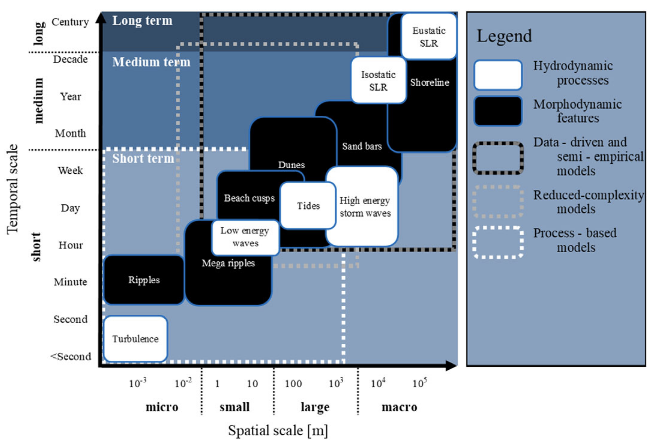
\includegraphics[width=0.8\linewidth]{images/spatial-and-temporal.png}
    \caption{A schematic diagram representing approximate spatial and temporal modelling scales that are appropriate to hydrodynamic processes (white box) and morphodynamic features (black box). Reproduced from Hunt et al. (2023) \textsuperscript{[5]}}
    \label{figure1}
\end{figure}

% Ocean waves produced from wind is the most prevalent coastal process

\par{Sedimentary erosion and accretion caused by hydrological processes derived from waves generated by wind blowing over large stretches of ocean is the predominant morphological influence on most coastal areas.~\textsuperscript{[5]}~\textsuperscript{[6]} As waves are generated over large fetches of ocean and propagate into the nearshore domain (the subaqueous zone commonly spanning 100m directly seaward of the shoreline) they dissipate as depth decreases to beneath their height or they reach the shore. Their energy is augmented by that of other hydrological processes occurring at different spatial and time scales such as tides, to dictate an overall circulatory and sedimentary gradient of the area, which in turn determines the composition of local morphologies, geologies, and ecologies. By this token, characterizing the hydrodynamics of the coastal zone is essential to understanding all other processes there, and by extension the ability to successfully develop methods for sampling them.~\textsuperscript{[7]}}

% ----- 1A. COASTAL PROCESSES - HYDROLOGY -----

\subsection{Hydrology}

% Diagram of marine processes, energy as a function of frequency

\begin{figure} 
    \centering
    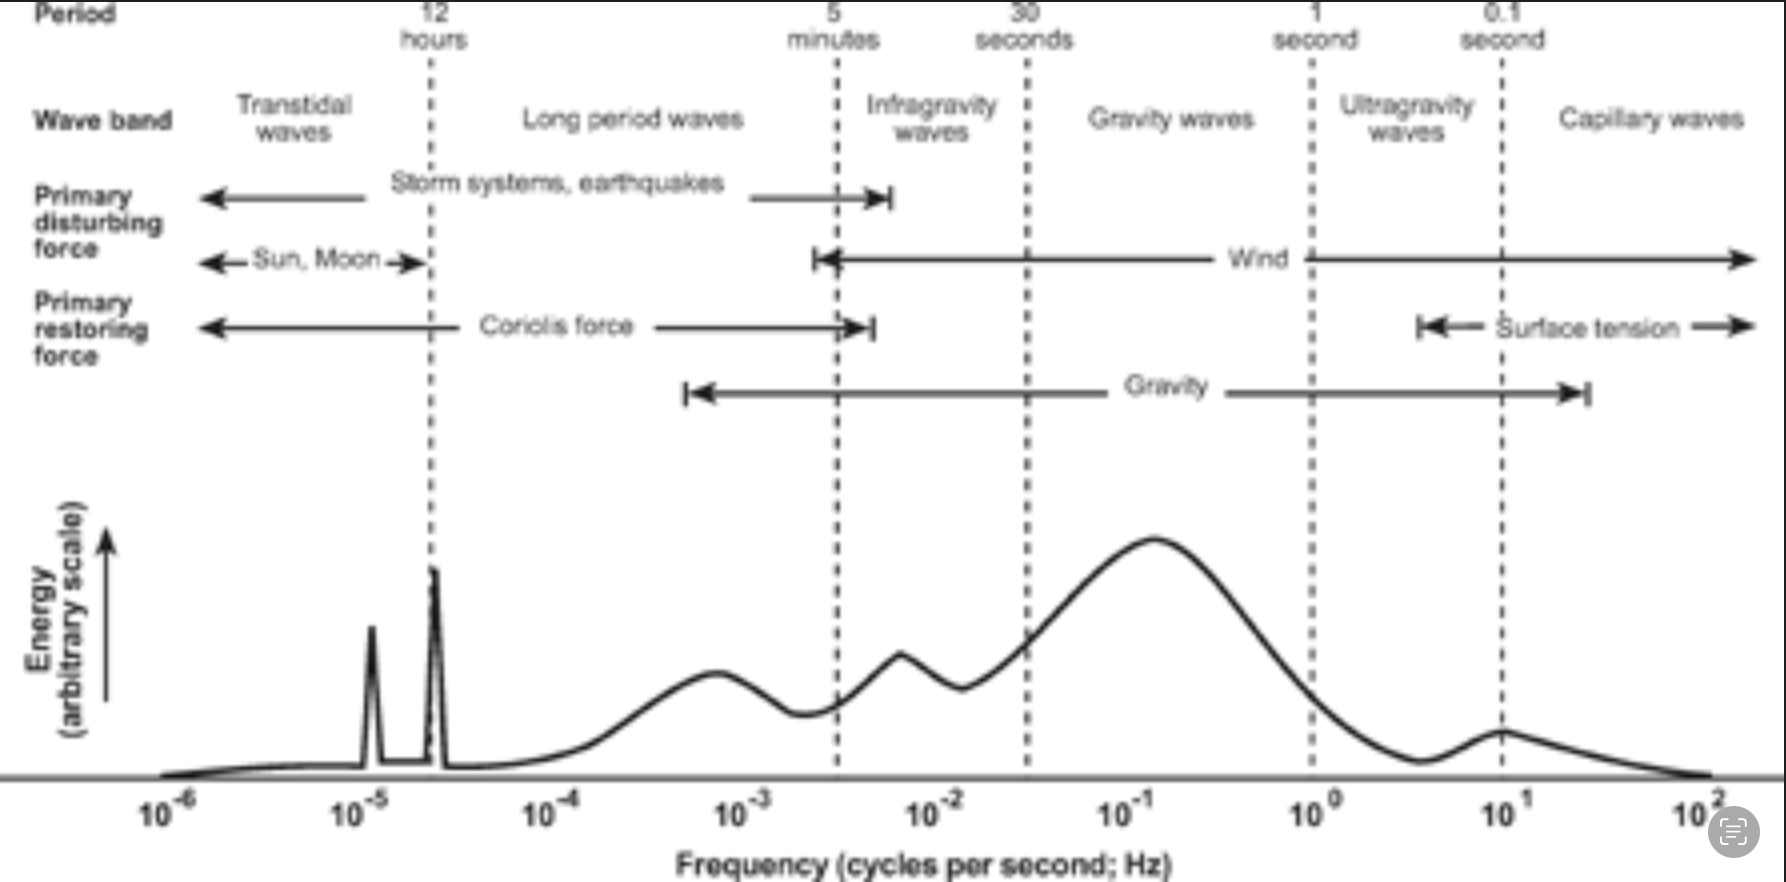
\includegraphics[width=1\linewidth]{images/ocean-wave-energy-schematic.png}
    \caption{Placeholder for self generated graphic based on this one from Kinsman, 1984\textsuperscript{[14]}}
    \label{figure2}
\end{figure}


% Wave generation from wind

\par{\hspace{.5cm}Ocean waves are created when a disturbing force acts on the ocean and a restoring force acts to restore equilibrium. These forces produce waves of varied frequency, wavelength, height, and direction.\textsuperscript{[6]}~\textsuperscript{[7]}~\textsuperscript{[11]}~\textsuperscript{[14]} The most commonly observable waves are wind waves: those generated by friction drag from wind blowing over an area of the ocean's surface, transferring energy into the to water.~\textsuperscript{[6]}~\textsuperscript{[7]}~\textsuperscript{[8]}~\textsuperscript{[9]}~\textsuperscript{[14]} A sea is area in which strong winds actively work to generate irregularly peaked waves of varied periodicity traveling in a broad spectrum of direction, resulting in a chaotic ocean surface. When energy losses from waves breaking are offset by energy gained from blowing wind, the sea is said to be fully developed or arisen.~\textsuperscript{[9]}~\textsuperscript{[14]}~\textsuperscript{[15]} The power spectra of a fully developed sea, first proposed by Willard Peirson and Lionel Moskowitz, is well defined, and allows forecasters to accurately model wave conditions based on wind speed and direction.~(\cref{figure3}).~\textsuperscript{[11]}~\textsuperscript{[15]}}


% More specific wave generation from wind

\par{To describe the processes by which wind generates waves more specifically, wind blowing over the ocean stretches the waters surface, and as surface tension works to restore it to equilibrium, capillary (low energy, short wavelength, high frequency) waves, are formed. As wind continues to blow, capillary waves are compounded by wind energy and grow. Capillary waves which exceed a wavelength threshold of 1.74cm become gravity waves, as gravity supersedes surface tension as the prevailing restoring force, and works to pull the crest of a wave downward. The water's inertia causes the crests to overshoot and become troughs, inducing a cycle in which water molecules oscillate in a near-frictionless orbit as gravitational forces work to restore the fluid to a state of equilibrium, allowing them to propagate long distances across the ocean's surface.~\textsuperscript{[6]}~\textsuperscript{[9]}~\textsuperscript{[11]} ~\textsuperscript{[14]} As wind activity ceases or waves move away from the area of generation, they are sorted into packets of uniform wavelength and direction. Gravity waves have a period around .1 Hz and represent the most energetic band of the spectra.~\textsuperscript{[6]}~\textsuperscript{[10]}~\textsuperscript{[11]}~\textsuperscript{[15]}.}


% Pierson-Moskowitz Graph, spectral plot of fully developed sea

\begin{figure}
    \centering
    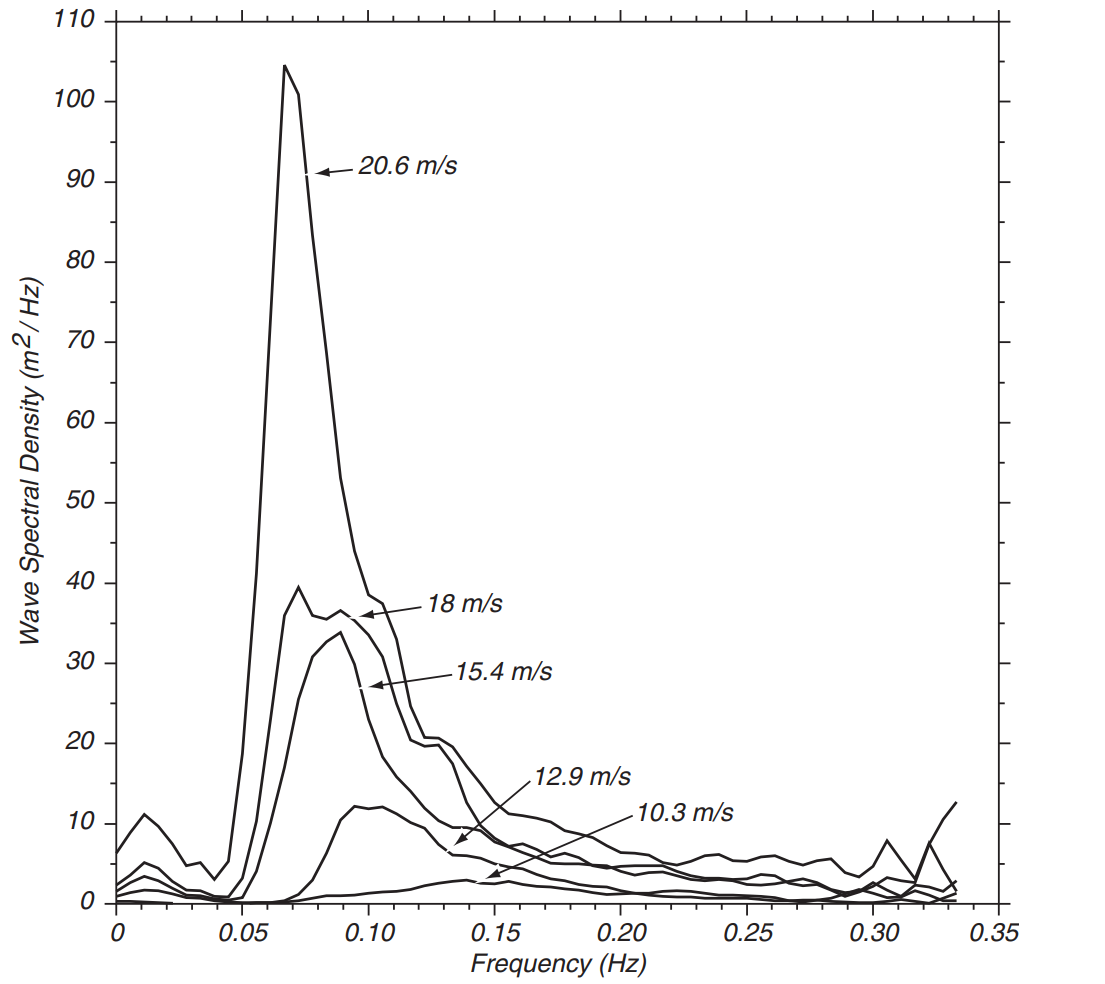
\includegraphics[width=0.75\linewidth]{images/developed-sea-power-spectrum.png}
    \captionof{figure}{Placeholder for self generated version of this Pierson-Moskowitz spectral graph.}
    \label{figure3}
\end{figure}
    
% Propagation across ocean to coasts

\par{All ocean waves propagate across the surface of the ocean as potential energy which is released as kinetic energy as they shoal through contact with bottom morphologies and are broken by spatial features of the nearshore zone and shoreface.~\textsuperscript{[6]}~\textsuperscript{[7]}~\textsuperscript{[9]} Gravity waves (10s) compound with phenomena occurring at longer time scales such as infragravity waves (30s - 300s), as well as tidal modulation and resulting instabilities from longshore currents (10\textsuperscript{2}-10\textsuperscript{3}-s), to create the full spectrum of nearshore gravity-based wave activity.~\textsuperscript{[7]}~\textsuperscript{[9]}~\textsuperscript{[12]}~\textsuperscript{[13]} Extreme events such as tsunamis generated by seismic activity and seiche (resonant rocking of water produced by sudden change in atmospheric pressure) may produce and augment nearshore wave activity episodically.~\textsuperscript{[7]}}

% Tides

\par{Tides are another marine process that has a significant effect coastal areas, causing variation in sea level that augments wave activity and causes seawater to inundate and receed from low-lying areas, generating currents. The disturbing forces which generate tides are gravitational forces from the moon and sun which act on a rotating earth, causing global variation in local ocean surface height. Isaac Newton, in his work \textit{Principa Mathematica}, postulated the Equilibrium Theory of Tides, which described tides as two bulges of heightened sea level on opposite ends of the earth generated as the result of astrological forces acting upon the ocean's surface counter to earth's gravity.~\textsuperscript{[7]}~\textsuperscript{[9]}~\textsuperscript{[11]} Newton's theory was intentionally limited: it assumes infinitely deep oceans, not sufficient to explain how tidal wave height and length would exceed the extents of oceanic basins when considering the speed of solar and lunar positional change relative the earth.}

% More specific description of tides

\par{Pierre-Simon Laplace expanded upon Newton's Equilibrium Theory of Tides by formulating the Dynamic Theory of Tides, which additionally incorporated phenomenon such as friction, the earth's rotation, the Coriolis effect, and the shape of oceanic basins, to more accurately characterize tidal behavior.~\textsuperscript{[7]}~\textsuperscript{[11]} The Dynamic Theory of Tides describes tidal waves that circulate about amphidromic points, where the tidal range is zero, counterclockwise in the Northern Hemisphere and clockwise in the Southern. Models incorporating these principles have been successful in predicting tides in accordance with observed behaviors.~\textsuperscript{[7]}~\textsuperscript{[11]}  When observed locally, tides are visible through the shoreline fluctuation between low and high tide once (diurnal) or twice (semidiurnal) daily depending on location relative to amphidromic points. These shifts generate longshore currents parallel to all coasts, and cross shore currents where tidal floods and ebbs rush into and out of enclosed areas such as estuaries and other inlets.~\textsuperscript{[7]}~\textsuperscript{[9]} In coastal areas sheltered from high wave energy, tidal activity can dominate local sediment transport, and exhibit significantly different physical and biological attributes from those predominantly effected by wave activity.~\textsuperscript{[11]}}

% Chappell and Shackelton graph, eustatic sea level change

\begin{figure}
    \centering
    \includegraphics[width=0.75\linewidth]{images/eustatic-sea-level-change.png}
    \caption{Placeholder for self generated version of this graph from Chappell and Shackelton 1986.~\textsuperscript{[18]}}
    \label{figure4}
\end{figure}

% Eustatic sea level change

\par{The most infrequent hydrodynamic processes which effect coastal waters are those associated with eustatic sea level change, or cumulative changes in the volume of the ocean from factors which occur over periods of 10\textsuperscript{5} years or longer, such as addition of water through glacial melting and volcanic out-gassing, thermal expansion of water, and changes in the shape of the seafloor through sediment deposit and tectonic spreading.~\textsuperscript{[4]}~\textsuperscript{[6]}~\textsuperscript{[17]} Local isostatic changes of land level with respect to sea height is caused by tectonic uplift from decadal lithospheric convergence.~\textsuperscript{[6]}~\textsuperscript{[17]} These processes have the most significant influence on shoreline change over longer timescales.~\textsuperscript{[4]} Sea levels have been continuously rising for the past \textasciitilde20,000 years since the Last Glacial Maximum (LGM), primarily caused by the melting of ice sheets from the Late Pleistocene, and is the primary contributor today's coastal and inland hydrological features, through inundation of low-lying continental areas and exposure of areas formally eroded and covered by glacial ice in high latitudes~\textsuperscript{[6]}~\textsuperscript{[8]}~\textsuperscript{[17]}~\textsuperscript{[18]}~\textsuperscript{[19]}}

% Fluvial contribution to coastal hydrodynamics

\par{Fluvial systems also work to influence coastal processes at areas where fresh water is channeled into an outlet and mix with oceanic salt water to form an estuary.~\textsuperscript{[9]}~\textsuperscript{[20]}~\textsuperscript{[21]}~\textsuperscript{[22]} At a rivermouth, the turbulent jetstream formed by fluvial discharge flowing into an estuary may dominate local hydrodynamics, the flow structure and velocity of which are dictated by the geometry of estuarine basin and are highly subject to episodic phenomenon such as storm surges or flooding events.~\textsuperscript{[20]}~\textsuperscript{[21]}~\textsuperscript{[22]} Where present, fluvial processes combine with tidal and wave action to form the overall hydrological gradient of that coastal locale, and may serve as the prevailing circulatory factor in some coastal areas which are well-sheltered from highly energetic marine processes.~\textsuperscript{[9]}~\textsuperscript{[20]}~\textsuperscript{[21]}~\textsuperscript{[22]}}

% ----- 1B. COASTAL PROCESSES - MORPHOLOGY -----

\subsection{Morphology}

% Refined definition of coastal area to include extents, now given understanding of coastal processes

\par{\hspace{.5cm}More nebulous than defining the coastal zone's extents are defining those of its sub-areas which group to form the full cross-shore (seaward normal from the shoreline) profile of a coast. Earlier, we adopted a definition of the coast as being an area where sub-decadal oceanic processes influence local morphology through sediment transport, and so we will divide the coastal zone into discrete sections based on which marine processes effect that area, and by extension the nature of sediment transport that occurs there. Therefore, by our definition, the furthest extent of a coast is the outer boundary where ocean waves shoal through contact with bottom morphologies. The offshore areas exceeding that boundary are unaffected by wave-action induced sediment transport and thus not included in our definition of the coastal zone.~\textsuperscript{[2]}~\textsuperscript{[6]}~\textsuperscript{[9]}~\textsuperscript{[16]}}

% Coastal profile with sub-zone delineation

\begin{figure}
    \centering
    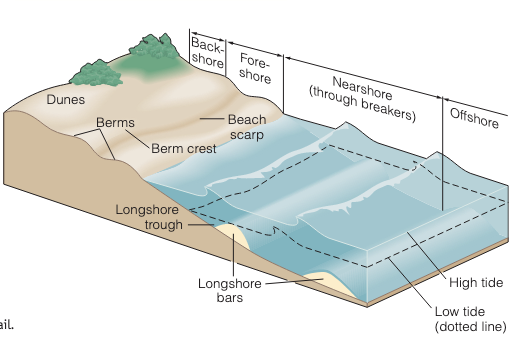
\includegraphics[width=1.0\linewidth]{images/coastal-sub-zones.png}
    \caption{Placeholder for self generated version of this infographic from Essentials of Oceanoraphy~\textsuperscript{[6]}}
    \label{figure5}
\end{figure}

% Coastal sub-zones

\par{Adjacent to that and proximal to the shoreline, is the littoral zone, the greater area in which sediment transport occurs both on in the water and on land.~\textsuperscript{[8]}~\textsuperscript{[16]} The littoral zone can be divided further into the nearshore, foreshore, and backshore areas~(\cref{figure5}). The seaward limit of the nearshore is the offshore boundary and extends to the shoreline. At the offshore boundary, waves shoal as depth becomes half the wavelength of incident wave, and break as they come into further contact with bottom morphologies in the surf zone, also included as a subsection of the nearshore. The foreshore is the section landward from the shoreline and extending to the high-high-water (HHW) mark, the extent to which the combination of tidal and wave activity reach.~\textsuperscript{[16]} Continuing landward, the backshore area begins at the HHW to the end of where loose sediment particles are deposited. Sediment in the backshore is subject mostly to daily aeolian transport, but can also be effected by episodic extreme wave and surge action from storms.~\textsuperscript{[2]}~\textsuperscript{[9]}~\textsuperscript{[12]}~\textsuperscript{[16]}}

% Map of Southern California littoral cells

\begin{figure}
    \centering
    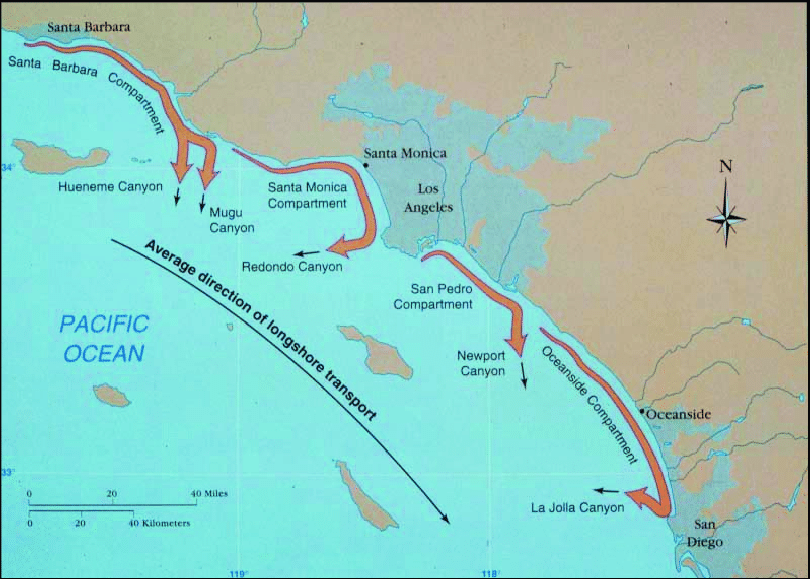
\includegraphics[width=.9\linewidth]{images/so-cal-littoral-cells.png}
    \caption{Placeholder for self generated version of this infographic from Littoral Cells in Southern California by Inman and Chamberlain ~\textsuperscript{[24]}}
    \label{figure6}
\end{figure}

% Classification based on sedimentary characteristics

\par{Sedimentary charactertistics serve as a useful classification scheme for coasts. One important distinction is between areas of coast which regularly experience a net gain in sediment accumulation as opposed to those which experience a net loss, cateogrized as either depositional and erosional respectively. Another distinction can be made based on the size of sediment grains present onshore, which ranges on a continuum from cliffs and large boulders, to rocks, to sand, to fine-grain mud.~\textsuperscript{[23]} Environments with different sedimentary characteristics exhibit vastly different geomorphic and biotic traits. Sedimentary characteristics are strongly correlated with energy from wave action: often coasts exposed to areas of high wave activity are erosional, as sediment becomes dislodged by wave energy and is transported by currents until it becomes deposited at sheltered beaches nearby.~\textsuperscript{[9]} The geometry of the littoral area also plays a factor: steepness and size of the foreshore and bathymetric gradients in the nearshore correlate to erosional rates and grain size. ~\textsuperscript{[8]}~\textsuperscript{[9]}~\textsuperscript{[16]}~\textsuperscript{[23]}}

% Segmentation based on sediment transport

\par{Segmenting coastlines according to sediment transport characteristics is also highly pertinent. A coastal or littoral cell is a contiguous sector of coastline in which erosional and accretionary processes are balanced, and spans the distance sediment is transported from an erosional source to the extent to which it is largely deposited or lost offshore.~(\cref{figure6}).~\textsuperscript{[9]}~\textsuperscript{[16]} The recognition of discrete littoral cells is essential to understanding and characterizing coastal morphological processes, and is regularly used as a tool in coastal land management and development.~\textsuperscript{[23]} Often littoral cells are bordered by clear geographic markers, such as headlands which restrict the angle of wave approach to the shoreline to disrupt the flow of sediment, and submarine canyons which channel sediments offshore.~\textsuperscript{[23]}~\textsuperscript{[24]} \par}

% Littoral cells and longshore transport

\par{A littoral cell experiences net transport of sediment in a single direction parallel to the shore.~\textsuperscript{[6]}~\textsuperscript{[16]} Waves refract in shallow water to break near-parallel to shore, but maintain a slight angle as they crash on the shoreface, resulting in Swash, a turbulent layer of onshore water.~\textsuperscript{[6]}~\textsuperscript{[28]} Swash rushes up the beach up at the angle of the breaking wave, then retreats straight down towards the shoreline due to gravity, during phases refered to as uprush and backwash respectively.~\textsuperscript{[6]}~\textsuperscript{[28]} Through uprush and backwash, sediment is loosened and then transported in a zig-zag pattern up and down the beach, with net direction parallel to the coast, in a collective process known as longshore drift.~\textsuperscript{[6]}~\textsuperscript{[28]} Local properties such as geographic location, shoreline irregularities, nearshore geometry, wind and wave energy, tidal currents, and sediment size, compound to influence how much sediment is removed, how quickly and in which direction sediment is transported, and where it becomes deposited.~\textsuperscript{[6]}~\textsuperscript{[8]}~\textsuperscript{[12]}~\textsuperscript{[16]}~\textsuperscript{[28]} Sediment will be continuously deposited and transported longshore until the drift is interrupted or diverted by shoreline irregularities at the end of a littoral cell.~\textsuperscript{[24]}}

% Pictures of erosional morphology

\begin{figure}
    \centering
    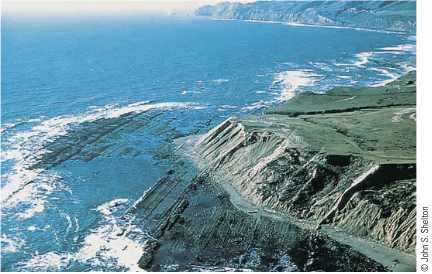
\includegraphics[width=.9\linewidth]{images/erosional-morphology.png}
    \caption{Placeholder for self generated version of this infographic from Essentials of Oceanography ~\textsuperscript{[6]}}
    \label{figure7}
\end{figure}

% Erosional features

\par{Coastal morphologies in the nearshore and foreshore are formed when sediment is removed or deposited as a result of hydrodynamic processes occuring over time, and so erosional coasts exhibit a different array of morphological features from depositional ones. Net sediment loss at erosional coasts expose bedrock directly to wave action. Waves erode bedrock by pushing air and water into small fissures which build pressure to fracture and dislodge debris. Additionally, waves may hurl debris, and water from waves may dissolve minerals in certain types of rock to contribute to erosion more effectively.~\textsuperscript{[6]} Erosion occurs mostly at the water line, so the bedrock may develop at notches at the water line.~\textsuperscript{[6]}~\textsuperscript{[16]}~\textsuperscript{[28]} Notching can cause the rock above to collapse to form a steep cliff~(\cref{figure7}), and may result in other formations, as weaker zones of bedrock are removed to form features within the cliff-side such as caves. The base of notches into a cliff-side at the low tide mark which may remain as the ceiling above collapses, leaving a large flat wave-cut platform of rock at the low-tide line which remains submerged and unaffected during higher tides Formations such as sea stacks and arches may remain beyond the shoreline as the weaker rock around them is removed.~\textsuperscript{[6]} Longshore currents transport sediment generated through these erosive processes until it is deposited in more sheltered areas such as nearby bays, or removed.~\textsuperscript{[6]}~\textsuperscript{[28]} }

% Fluvial sediment input

\par{Fluvial systems are the primary input for sediment into the coastal area, as loose soil particles derived mostly from rain-based erosion are transported downstream and into estuaries.~\textsuperscript{[8]}~\textsuperscript{[20]}~\textsuperscript{[23]}~\textsuperscript{[25]} In areas subject to high wave activity, sediment removed by wave action may exceed sediment deposited from fluvial processes, resulting in erosion.~\textsuperscript{[20]}~\textsuperscript{[26]} Tidal intrusion into estuaries creates currents which interact with jetsteams at the river-mouth and may create shear fronts and other complex flows which result in unique morphologies.~\textsuperscript{[6]}~\textsuperscript{[8]}~\textsuperscript{[27]} Watershed areas with low wave and tidal activity are more likely to experience sediment accumulation, which may result in depositional landforms such as deltas which penetrate into coastal waters.~\textsuperscript{[6]}~\textsuperscript{[8]}~\textsuperscript{[16]} Anthropic manipulation of watershed systems can also have a significant impact on fluvial sediment transport and deposition, as damming, dredging, and other forms of water management can alter the natural flow of sediment downstream.~\textsuperscript{[16]}~\textsuperscript{[26]}}

% Maps of transgressive dunefield evolution

\begin{figure}
    \centering
    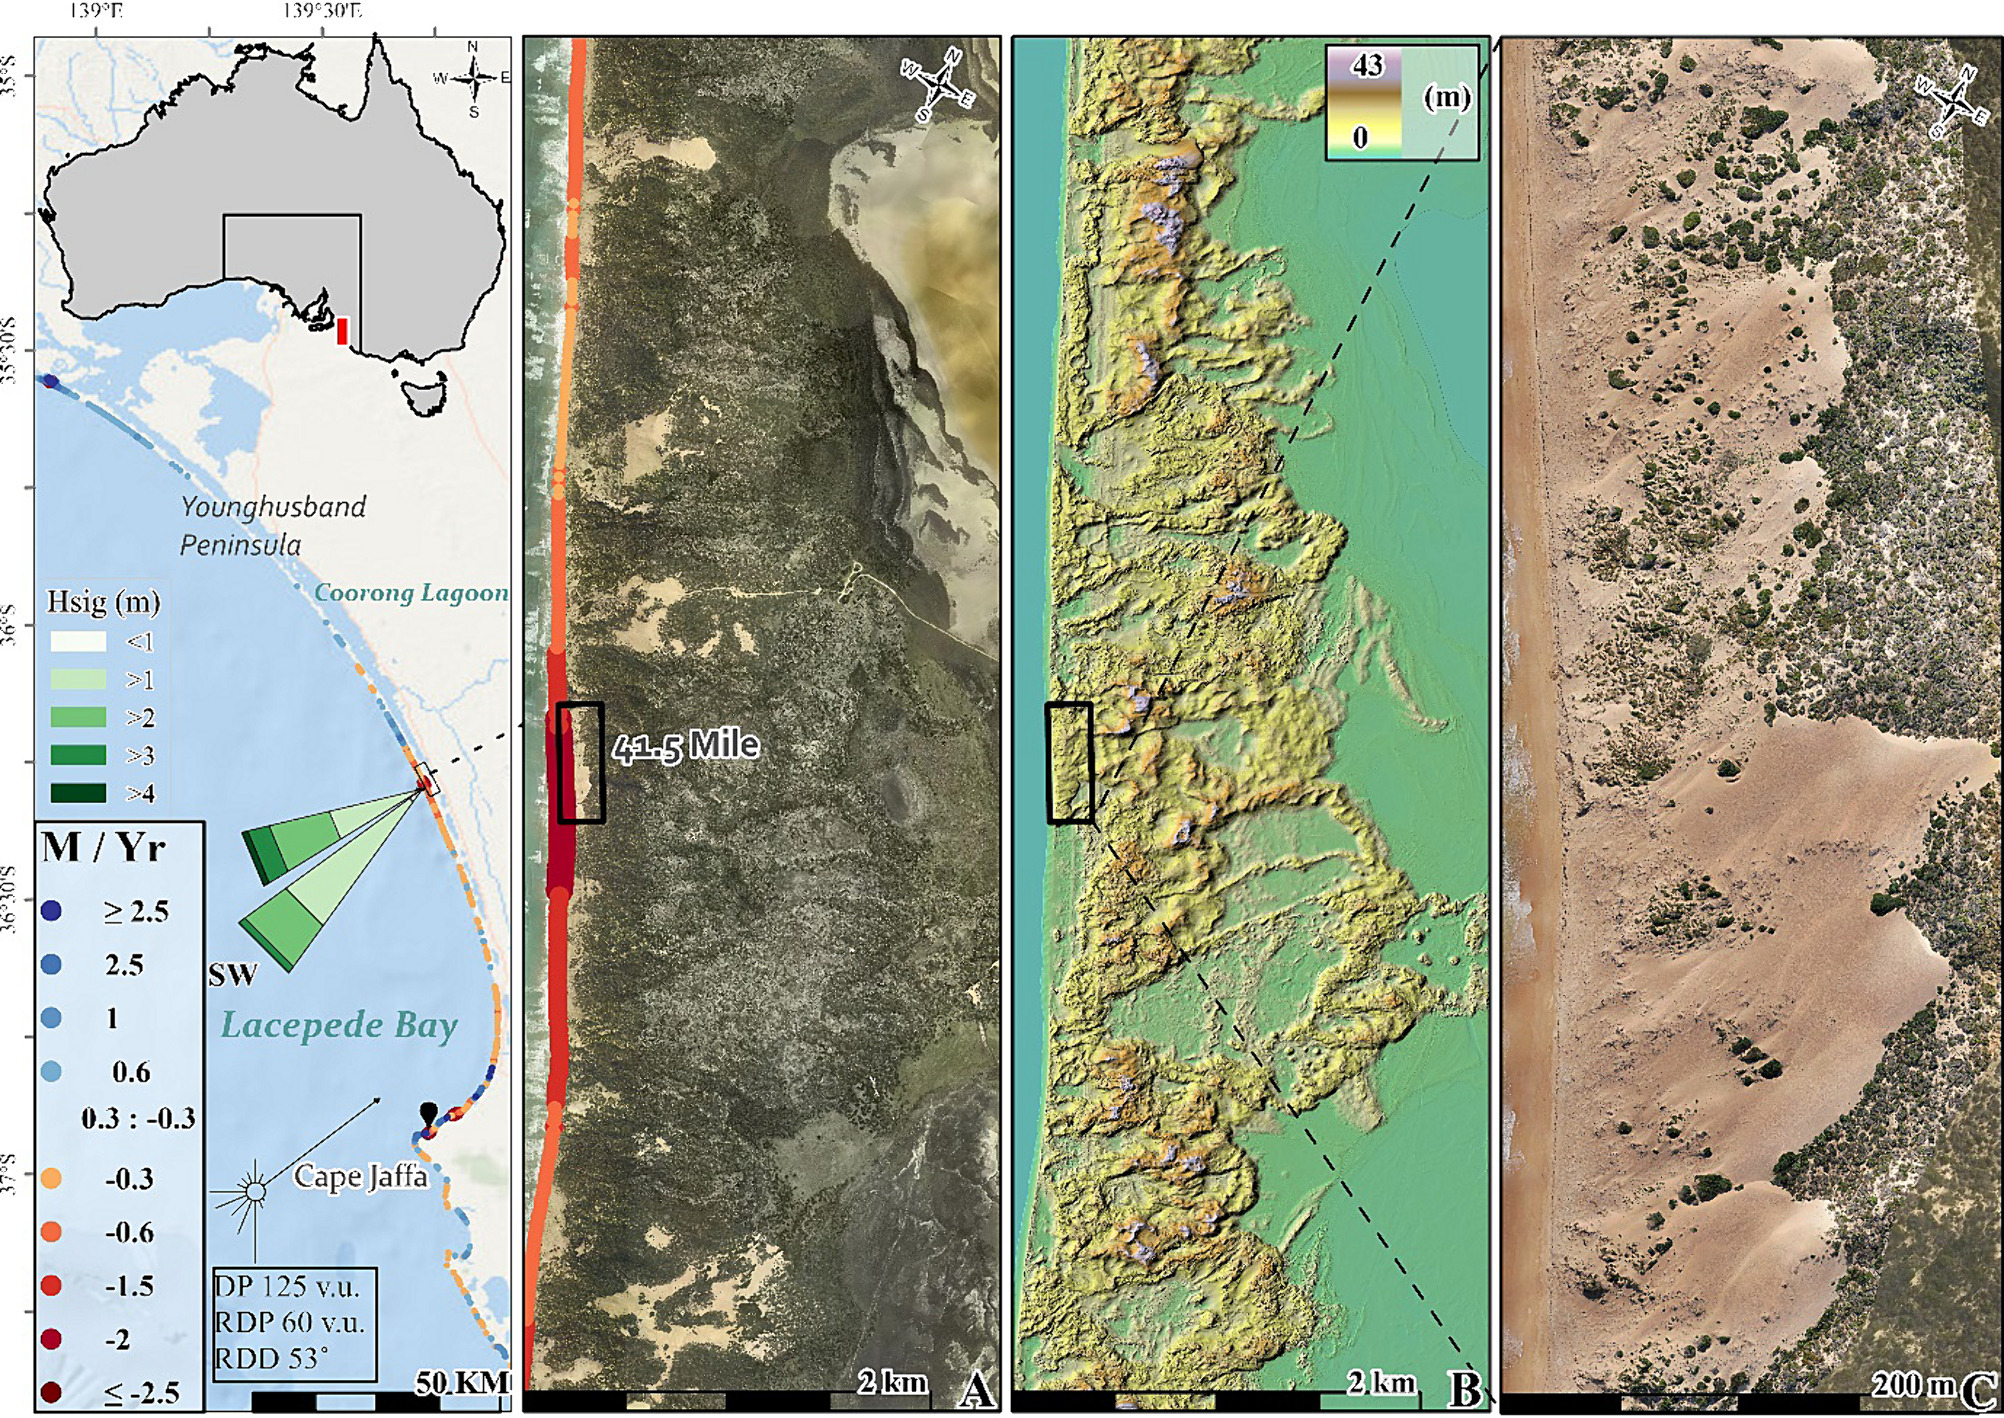
\includegraphics[width=.9\linewidth]{images/dunes.jpg}
    \caption{Placeholder for self generated version of this infographic from Coastal transgressive dunefield evolution as a response to multi-decadal shoreline erosion.~\textsuperscript{[16]}}
    \label{figure8}
\end{figure}

% Depositional features

\par{Most familiarly depositional coasts develop beaches, which is a zone of loose particles that covers the shore.~\textsuperscript{[6]} Beach particles may be generated from different sources—--many are generated from the processes described earlier, such as cliff erosion and fluvial discharge, but others in tropical regions are composed of biological particles such shells and fragments of coral, and in regions subject to volcanic activity may be composed to fragments of andesite or basalt from lava.~\textsuperscript{[6]}~\textsuperscript{[16]}~\textsuperscript{[26]} Particles can range in size from silt (0.0039-0.0625mm), to sand (0.0625-2mm), to pebbles and cobbles (0.5-256mm), to boulders (greater than 256mm), determined primarily by three factors: sediment source, wave-energy level, and offshore slope upon which the beach is constructed.~\textsuperscript{[26]} A single beach is composed of grains of many different sizes which become sorted through wave action, creating a strong correlation between mean grain size and wave energy level both up and offshore.~\textsuperscript{[26]} Beaches develop distinguishable morphologies induced by the marine processes to which they're exposed---the extent of wave and tidal action often creates a accumulation of sediment parallel to the shoreline called a berm, which marks the boundary between the fore and backshore areas.~\textsuperscript{[6]}~\textsuperscript{[26]} Scarps are formed at the same boundary, but instead when erosional wave action removes sediment to form a steep cliff.~\textsuperscript{[6]}~\textsuperscript{[26]}~\textsuperscript{[30]} Landward from that boundary, backshore areas commonly feature dunes formed through aeolian transport of sediment from surrounding sources.~\textsuperscript{[16]} Coastal dunes systems are highly complex environments that are the sole subject of more focused study, but in short summary their structure is primarily dependent on their ability to host vegetation and hold moisture to maintain stability and protect from erosion.~\textsuperscript{[16]} Dune systems exist on a continuum from highly stable to unstable and ephemeral~(\cref{figure8}), the later given the adjective transgressive.~\textsuperscript{[16]}~\textsuperscript{[31]} Where vegetation is present, dune systems become divided into primary and secondary subsections---the primary section features foredune, }

% Diagram of longshore bars

\begin{figure}
    \centering
    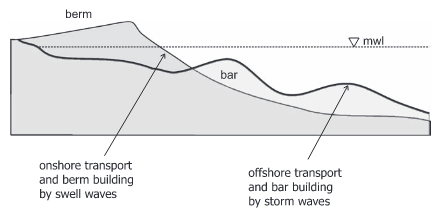
\includegraphics[width=.9\linewidth]{images/barred-profile.png}
    \caption{Placeholder for self generated version of this infographic from Introduction to Coastal Processes and Geomorphology. ~\textsuperscript{[16]}}
    \label{figure9}
\end{figure}

% Longshore bars

\par{Depositional beaches commonly feature subaqueous accumulations of sediment near-parallel to shore in the nearshore area, referred to as longshore bars~(\cref{figure9}). Longshore bars are an important area of study because of their influence on local hydrodynamics, through dissipation of wave energy offshore and contribution to local circulatory patterns.~\textsuperscript{[6]}~\textsuperscript{[16]}~\textsuperscript{[29]} The profile of barred coastlines may diverge from one another in several ways, for example---the amount of bars and how they are grouped, their location with respect to the shoreline, and the shape, slope, and stability of individual bars. ~\textsuperscript{[29]}~\textsuperscript{[32]} Several hydrological and geometrical factors contribute to the morphological characteristics of longshore bars, the most notable of which are---sediment transport from wave-induced currents such as longshore drift counter to flows from offshore-flowing undertow, deformation of bottom sediment from standing infragravity waves, the range and frequency of tidal variation, and the slope of the near and foreshore areas, among others.~\textsuperscript{[6]}~\textsuperscript{[16]}~\textsuperscript{[29]} The ability of bars to maintain stability over timescales of days and weeks suggests their positionality and form represent the equilibrium between local hydrodynamic forces.~\textsuperscript{[16]} On average, bars migrate toward and weld to the beach as wave conditions calm, and migrate offshore during storms.~\textsuperscript{[16]}~\textsuperscript{[29]}}

% Labeled diagram of depositional morphologies

\begin{figure}
    \centering
    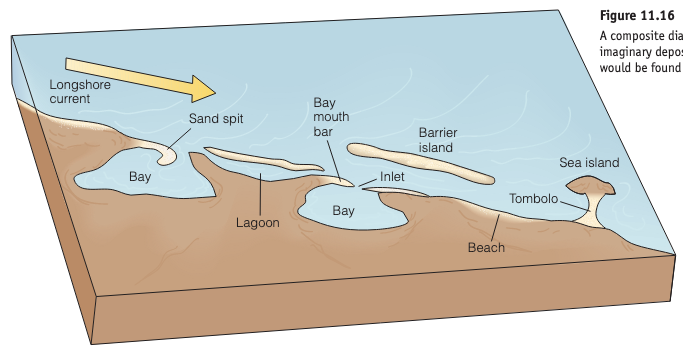
\includegraphics[width=.9\linewidth]{images/depositional-morphology.png}
    \caption{Placeholder for self generated version of this infographic from Essentials of Oceanography ~\textsuperscript{[6]}}
    \label{figure10}
\end{figure}

% Barrier systems

\par{Sediment which accumulates sub-aqueously in the nearshore may over-time emerge as barrier systems with an additional sub-aerial component, usually at the end of a littoral cell.~\textsuperscript{[6]}~\textsuperscript{[16]} The barrier may fully or partially trap water between itself and the mainland, to form unique features of full or mixed-saltwater composition but are largely shielded from marine processes, including---aquatic features such as lagoons, shallow bodies of salt water that have become partially or fully enclosed, and semi-aquatic ones such as intertidal mudflats, areas that become periodically inundated by and drained of saltwater through tidal action.~\textsuperscript{[6]}~\textsuperscript{[16]} Large-scale depositional features acting as barriers can be sub-categorized according to the nature of their attachment or independence from the mainland~(\cref{figure10})---barrier islands are fully separated from the mainland through sediment accumulation on submerged rises parallel to the shoreline.~\textsuperscript{[6]}~\textsuperscript{[16]} Sand spits form where longshore current slows as it clears a headland and approaches a sheltered bay, creating a peninsula of deposited sediment.~\textsuperscript{[6]}~\textsuperscript{[16]} Sand spits may close to form bay mouth bars, which then may become broken by when subjected to high wave or tidal energy, reconnecting the bay to the ocean through an inlet.~\textsuperscript{[6]} Tombolos may form as a bridge between islands and the mainland.~\textsuperscript{[6]}~\textsuperscript{[16]} The depositional nature of these features, in that they lack firm central cores as do islands that were once part of the mainland, makes them highly subject to erosion and migration.~\textsuperscript{[6]}~\textsuperscript{[16]}} 

% Estuaries

\par{Estuaries are partially or fully sheltered aquatic bodies of mixed salt and fresh-water composition, which occur at the coast where fluvial discharge interfaces with the ocean~(\cref{figure11}).~\textsuperscript{[6]}~\textsuperscript{[8]} Estuaries are often at the focus of coastal sciences, as they represent some of the most highly dynamic and productive coastal environments.~\textsuperscript{[8]} They are generally sheltered from wave action, but may be subject to daily tidal inundation and recession of varying degrees.~\textsuperscript{[8]} Estuarine bodies beg further sub-classification, as they can hold drastically different physical and ecological properties according to their origin.~\textsuperscript{[6]} Generally, they may be classified into four types---the most common of which are drowned river mouth inundated as an effect of eustatic sea since the last LGM.~\textsuperscript{[6]} Bar-built estuaries are partially or fully enclosed by barrier systems which limit tidal access and provide shelter from waves.~\textsuperscript{[6]} In mountainous areas of higher latitudes, glaciers formed during the Pleistocene eroded valleys into deep u-shaped troughs, and have since retreaded, allowing saltwater to be introduced and create fjords, long narrow marine inlets with steep sides.~\textsuperscript{[6]} Finally, tectonic subsidence at the coast can flood with seawater and mix with local freshwater sources to become an estuary.~\textsuperscript{[6]} The relative mixture of fresh and seawater has a significant effect on the ecology of an estuary, and also serves as an important classifier which will be discussed at length later on.~\textsuperscript{[6]}~\textsuperscript{[8]}}

% Pictures from estuaries

\begin{figure}
    \centering
    \includegraphics[width=1\linewidth]{images/cop-bar.JPG}
    \caption{An estuary at Coal Oil Point Reserve in Goleta, California, here sheltered from the ocean by a sedimentary bar, but is occasionally exceeded by tidal and wave action.}
    \label{figure11}
\end{figure}

% Biologically induced morphology

\par{Coastal zone biota, where present and abundant, have a significant effect on local geomorphology. Mangroves and seagrass protect coastlines from erosive processes and enhance accretion---roots and branches encourage the settling of fine-silts, attenuate wave action, and dampen current velocities, while fallen detritus increases the organic matter of sediments.~\textsuperscript{[16]}~\textsuperscript{[33]}~\textsuperscript{[34]} Coral reefs act as a natural breakwater to dissipate wave energy (on average \textasciitilde97\%) away from shore, protecting coastal areas from daily erosion from marine processes and episodic extreme erosion from natural disasters.~\textsuperscript{[35]}~\textsuperscript{[36]}~\textsuperscript{[37]} Coral reefs trap sediment, which may pile above the HHW to develop a sub-aerial component and form a cay---an island which may eventually become host to vegetation and soil.~\textsuperscript{[38]} Coral reefs barriers can also form lagoons. Later on, we will conversely discuss geomorphological influences on biological zonation as well.  }

% Geographical effects on erosional / depositional: Trialing edge, roaring 40s, etc...

% ----- 1C. COASTAL PROCESSES - ECOLOGY -----

\subsection{Ecology}

% ----- 1D. COASTAL PROCESSES - ANTHROPOLOGY -----

\subsection{Anthropology}

% History of human civilization at the coast
% Economies of the sea
% Recreation
% Population rise in LECZ
% Climate change induced SLR
% Coral bleaching, harmful algae blooms
% Flooding
% Hard infrastructure: jetties, dykes, etc.
% Soft infrastructure: Reefs, grasslands, etc.

% ----- 2. SAMPLING AND MODELING -----

\section{Sampling and modeling}
\fancyhead[C]{SAMPLING AND MODELING}

% Challenges with in-situ sampling

\par{The dynamic processes that the coastal area is subject to makes it a difficult environment to sample, particularly in the surf-zone where wave and current action, as well as the sediment transport they induce, render the area unstable for traditional in-situ instrumentation.~\textsuperscript{[7]} Obtaining data from subaqueous platforms carries unique challenges in the way of connectivity to power and internet infrastructure.~\textsuperscript{[7]} The processes and features of interest have large spatial extents, and are mostly inhomogeneous both across and alongshore, so sampling at the resolution necessary to fully characterize them would require a large array of in-situ point sensors.~\textsuperscript{[7]}}

% Remote sensors as a solution to challenges

\par{Remote sensors are those aquire information about a thing at a distance by detecting propagated signals. Measurements are made by detecting and measuring changes imposed by the subject on incident fields. Two important classifiers for remote sensors are active and passive. Active sensors, such as LiDAR and RADAR, are those that emit a signal and measure the time for it takes for that signal to reflect off of a surface and return. Passive sensors, such as optical and thermal cameras, gather electromagnetic radiation that is either emitted by an object or generated from another source and reflected off of an object.~\textsuperscript{[39]}~\textsuperscript{[40]} Most remote sensors produce a two-dimensional array of values---i.e images---gathered from a grid of detectors, enabling simultaneous sampling of values across a spatial extent and encode spatial information.~\textsuperscript{[40]} The ability of remote sensors to collect data away from harsh marine environments and provide spatial information make them an effective alternative to in-situ devices for measuring environmental parameters in the nearshore zone.~\textsuperscript{[7]}}

% Retrieval algorithms

\par{Retrieval algorithms are needed to extract information about the state of environmental parameters from the data collected by remote sensors.~\textsuperscript{[7]} Accurate representation of geophysical phenomena requires raw image data to be subject to some transformation function consisting of a series of sub-functions, which may include---filtering, normalization, spectral analysis, or assimilation of data from one sensor with that of other types.~\textsuperscript{[7]}~\textsuperscript{[41]}~\textsuperscript{[42]}~\textsuperscript{[43]}~\textsuperscript{[44]}}

% Tradeoffs between platforms
% ***** NOTE: Rewrite the end of this paragraph about spaceborne remote sensing. *****

\par{Remote sensors can be deployed from a variety of platforms, they may be: mounted at fixed locations, on manned or unmanned air and watercraft, or on satellites.~\textsuperscript{[7]} The most significant tradeoff between platforms is between dwell and footprint, the length at which data is gathered from one area versus the size of the total area from which data is gathered.~\textsuperscript{[7]} A certain amount of dwell or footprint may be necessary for some retrieval algorithms and not for others.~\textsuperscript{[7]} A common platform for remote sensors, and that which perhaps carries the strongest association to remote sensing as a discipline, are spaceborne satellites, from which the vast majority of remote sensing data is captured. Resolution is an important factor to consider when using remote sensing data from satellites, for example---the National Aeronautics and Space Administration (NASA) Landsat program offers an extensive database of high-quality imagery taken by rigorously calibrated instruments mounted on satellites that is free and open, making it an ideal source of data for many scientific applications.~\textsuperscript{[45]}~\textsuperscript{[46]} However, each pixel of an image captured from a Landsat satellite represents 30 square meters of the earth's surface, and an image is captured for a given area every 16 days, so Landsat imagery does not meet the spatial or temporal requirements needed to characterize some of the processes of interest to coastal science detailed earlier.~\textsuperscript{[45]}~\textsuperscript{[46]} These tradeoffs, among others, are important to consider when deciding which datasets are suitable for a specific use-case, or applying constraints to a bespoke remote sensing system.}

% ----- 2A. TECHNOLOGY -----

\subsection{Technology}

% How remote sensors are classified

\par{There are more specific classifiers for remote sensors that are distinguishable from one another according to the signals they detect, which properties of those signals are measured, and the output representation of that information. A single remote sensing device may exhibit several classifiers, and some classifiers share overlapping features with one another.}

% Intro to electromagnetic imaging sensors, photographic camera

\par{The most well represented remote sensors are imaging sensors of electromgnetic radiation---those which acquire two-dimensional arrays of radiant intensity values from the incident electromagnetic field. The first and most omnipresent imaging sensor is the photographic camera, which acquires optical images of visible light, or radiant energy from the visible band of the electromagnetic spectrum.~\textsuperscript{[48]}~\textsuperscript{[49]}~\textsuperscript{[50]} The first photograph was taken by Daguerre and Niepce in 1839, and one decade later in 1849, Colonel Aimé Laussedat of the French Army Corps of Engineers developed a program to use oblique photography for topographic mapping.~\textsuperscript{[48]}~\textsuperscript{[50]}  The next decade, Gaspard Tournachon took photographs of Paris from a hot-air balloon looking straight down at the ground, marking the beginning of vertical airborne photography, the technique most commonly associated with remote sensing.~\textsuperscript{[48]}~\textsuperscript{[50]}}

% Graph of broad electromagntic radiation bands

\begin{figure}
    \centering
    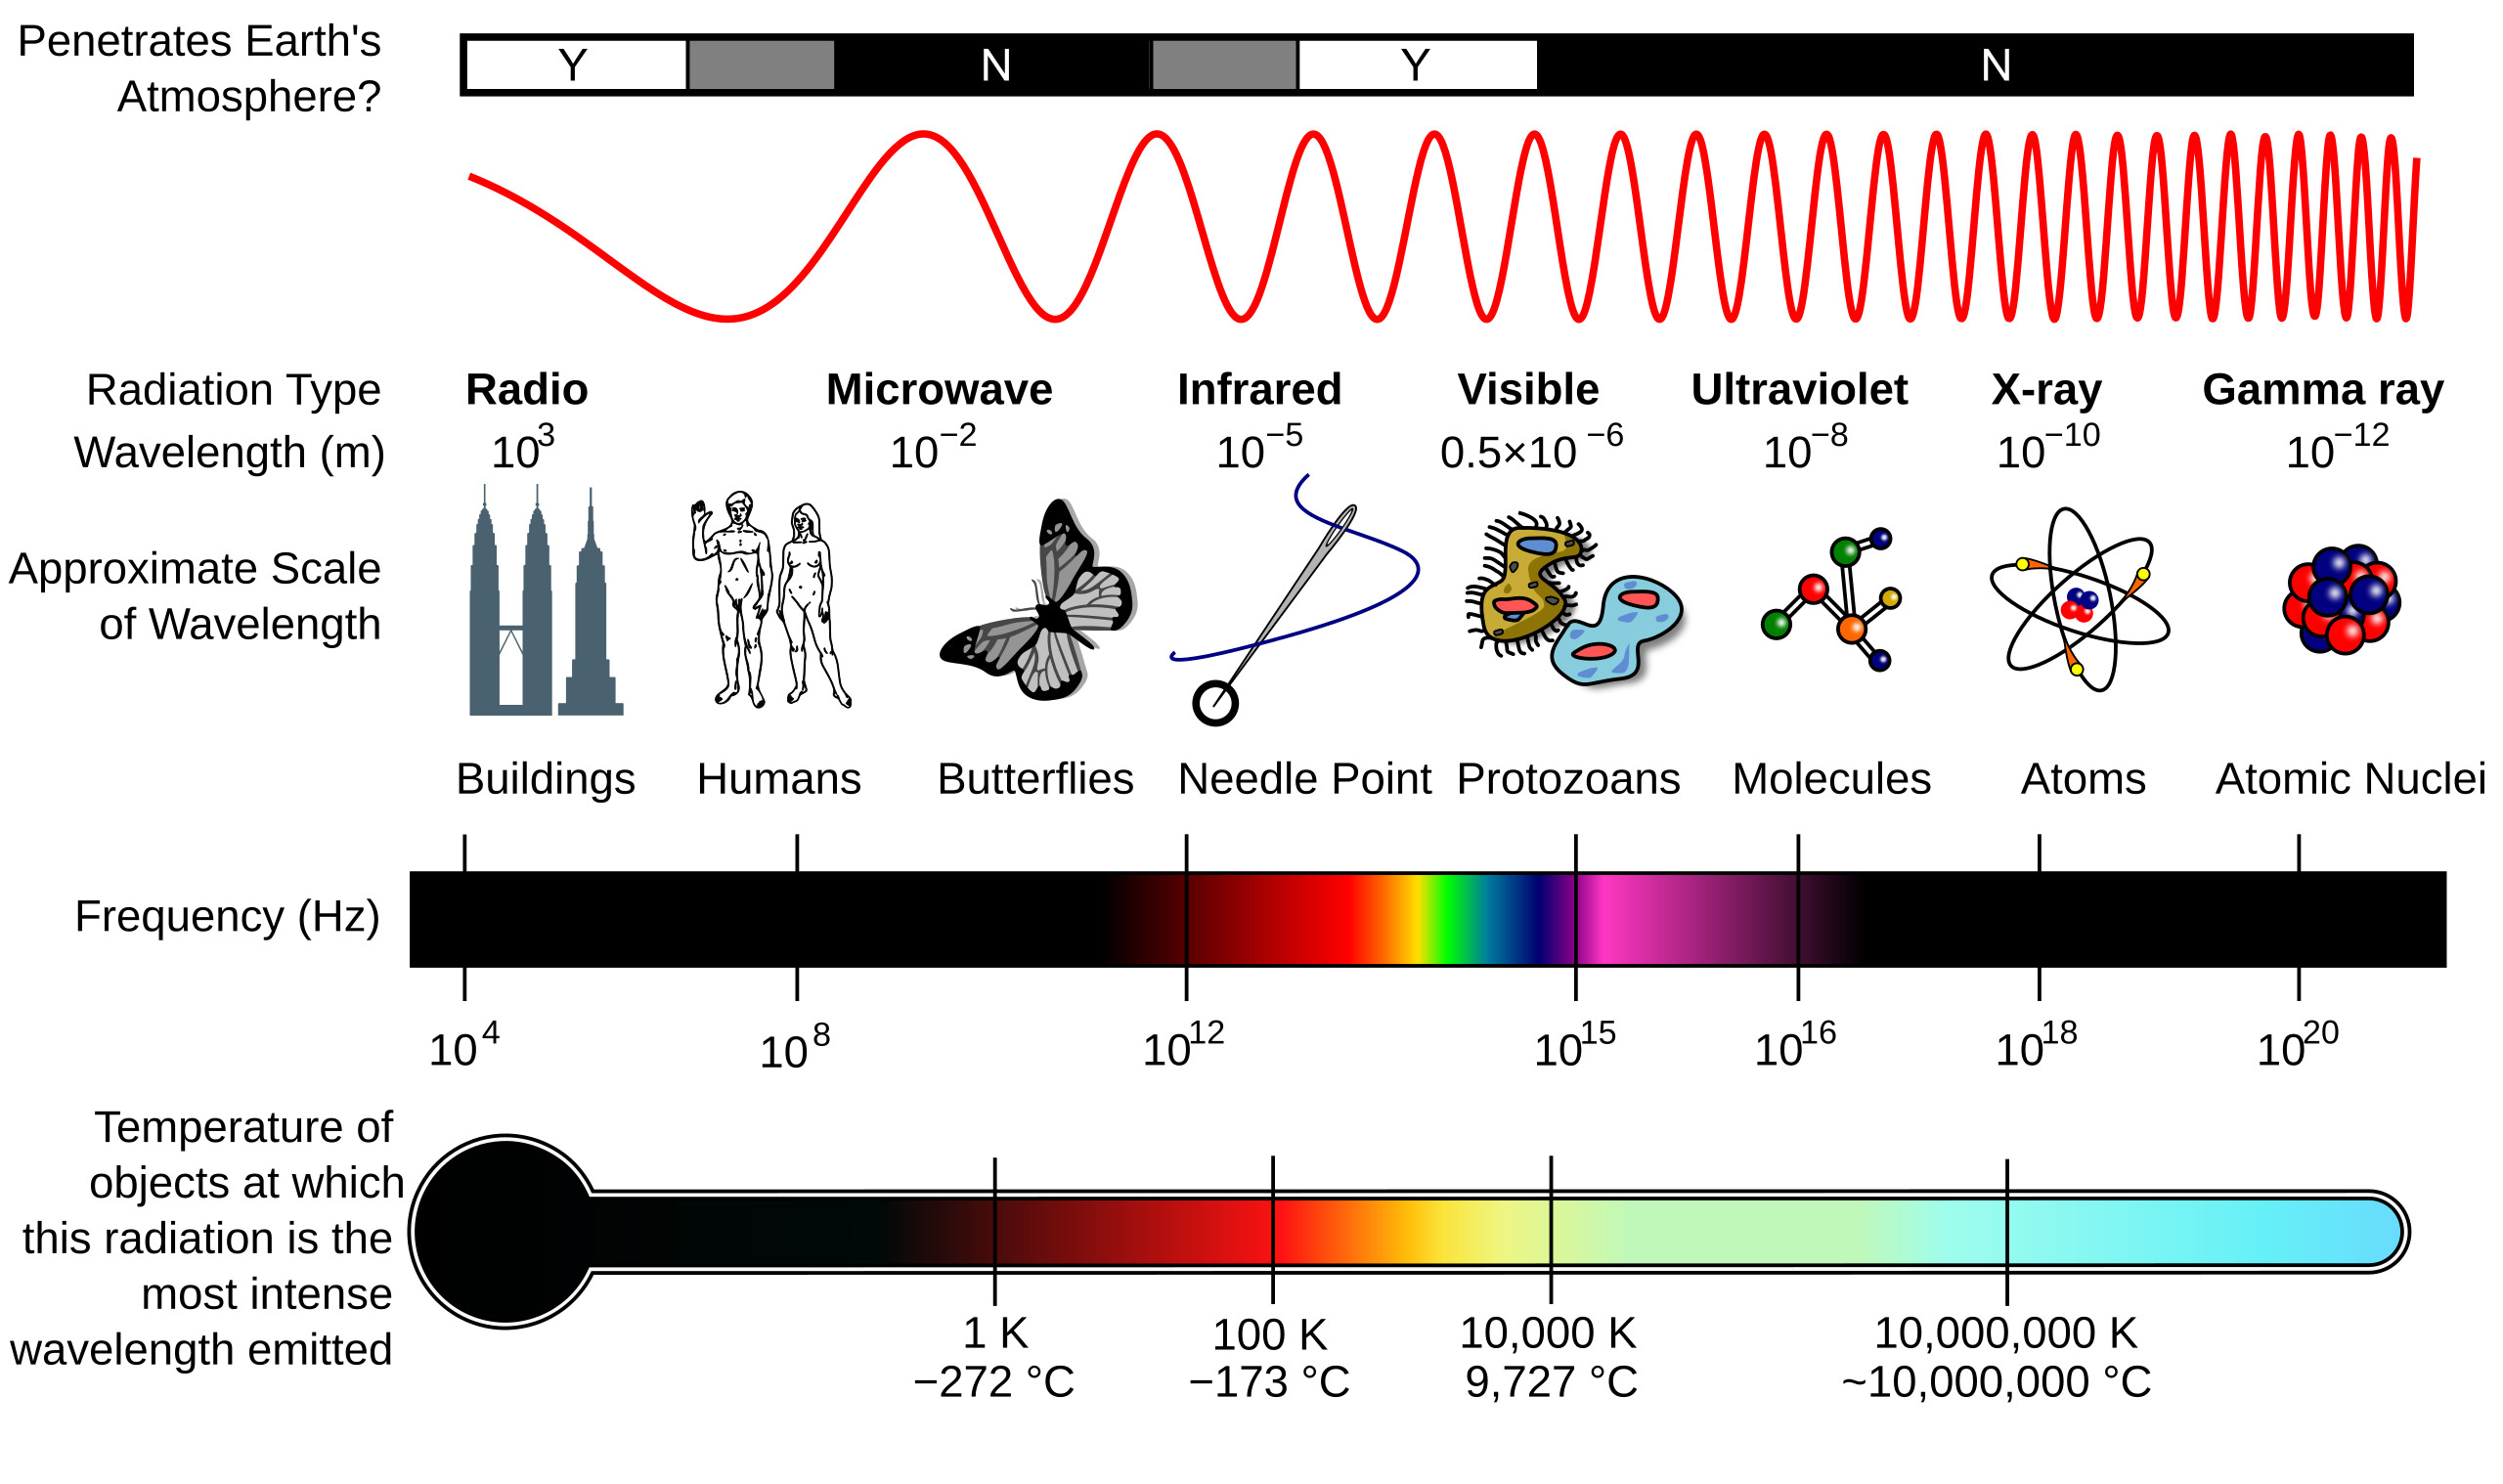
\includegraphics[width=1\linewidth]{images/em-spectrum.png}
    \caption{Placeholder for self generated version of this chart from NASA.}
    \label{figure12}
\end{figure}

% Landsat to introduce multispectral imaging

\par{In the mid-twentieth century, NASA sponsored studies toward applications for multispectral imaging in a leadup to the creation of the Landsat program in 1967.~\textsuperscript{[46]}~\textsuperscript{[48]}~\textsuperscript{[50]} Landsat is a joint NASA / USGS program to monitor terrestrial land use from a satellite that deploys a multispectral scanner, the first iteration of which was launched in 1972, and has since captured millions of mutlispectral images of the earth's surface, providing a continuous record of Earth's land for over half a century.~\textsuperscript{[45]}~\textsuperscript{[46]}~\textsuperscript{[51]} As mentioned earlier, Landsat represents one of the most robust and comprehensive remote sensing databases that enables research across multiple fields, but does not meet the spatial or temporal resolution required to characterize some of the most essential processes at the focus of coastal science. In order to impose necessary constraints, previous iterations of Landsat oriented toward land-use applications due to technological restrictions excluded bands capable of gathering information about aquatic bodies.~\textsuperscript{[55]}~\textsuperscript{[56]} However, the most recent iterations, Landsat 8 and 9 include technologies that are able to monitor important biogeochemical properties of shallow coastal waters, which we will visit in depth later on.~\textsuperscript{[53]}~\textsuperscript{[54]} Regardless, the Landsat program is especially worth mentioning here due to the program's historic role in launching a revolution in electronic imaging technologies, and because it continues to offer openly and easily accessible information on the most cutting-edge and rigorously calibrated remote sensors and sensing techniques.}

% Multispectral imagers

\par{Multispectral imagers are able to capture images from broad bands of the electromagnetic spectrum aside from the visible band, such as the microwave, infrared, and ulraviolet bands.~\textsuperscript{[48]} Filters divide the full spectrum from the incident field of electromagnetic radiation into broad bands with extents determined by a correlation between radiant intensity in a specific band to phenomena of interest.~\textsuperscript{[45]}~\textsuperscript{[48]} For example, the Landsat Operational Land Imager divides the infrared band (0.7-300μm) into the following more narrow bands---Near Infrared (NIR, 0.7-1.5µm) used for measuring vegetation health and biomass coverage, and Short Wavelength Infrared (SWIR, 1.5-3µm) used to measure soil moisture and detect minerals.Each band is exposed to a wafer of detecting elements which measures the intensity of the incident electromagnetic radiation across a spatial extent.~\textsuperscript{[53]}~\textsuperscript{[54]} Certain bands are excluded, as radiation at these wavelengths are particularly subject to absorption and scattering by the earth's atmosphere, and are not accessible to satellite-based remote sensing.~\textsuperscript{[53]}}

% NASA satellite bands chart

\begin{figure}
    \centering
    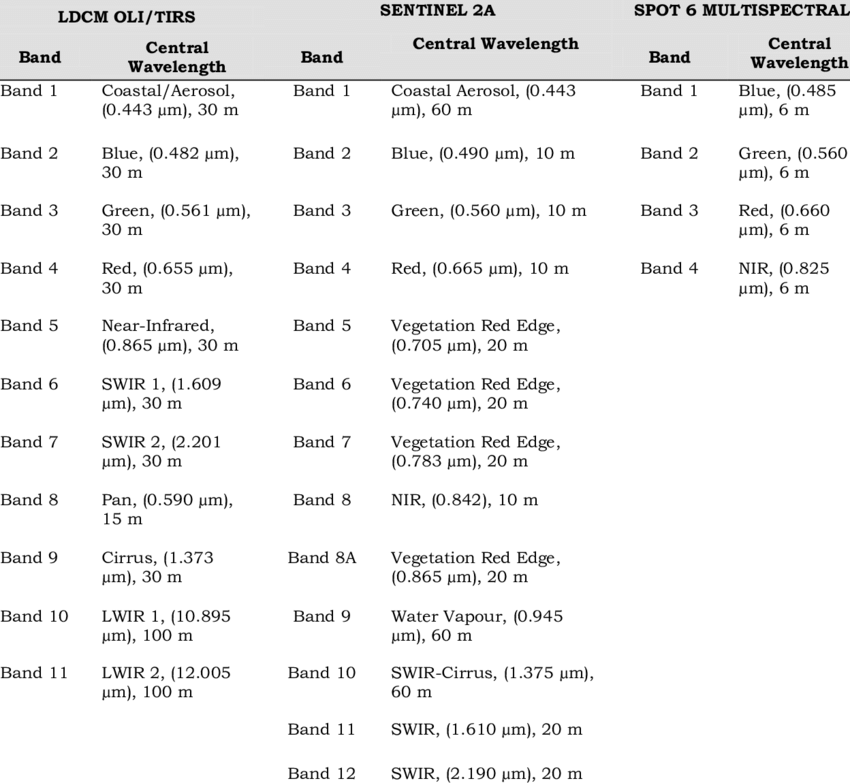
\includegraphics[width=0.7\linewidth]{images/landsat-8-specs.png}
    \caption{Bands available through NASA Landsat 8 and 9 Operational Land Imager and Thermal Infrared, as well as instrumentation on the Sentinel 2A and SPOT 6 satellites.}
    \label{figure13}
\end{figure}

% Challenges with sensing aquatic environments

\par{Aquatic environments pose a unique problem to being sampled from radiant sensors: water absorbs and scatters light, which is especially true for highly turbid waters in middle-to-high latitude coastal areas, which causes signals from aquatic areas to be weak or missing.~\textsuperscript{[55]}~\textsuperscript{[56]} Especially pertinent to our scope are new developments with the Operational Land Imager device mounted on the most recent Landsat 8 and 9 satellites, which is sensitive to low-frequency information from the blue / violet section of the visible spectrum, enabling it to sample color. For purposes of the Landsat program, this band is titled Coastal / Aerosol Band 1, as per it's primary usage, which is to monitor shallow-water for coloring agents---chlorophyll, total suspended solids (TSS), and yellowing colored dissolved organic materials (CDOM)---and atmospheric aerosols.~\textsuperscript{[46]}~\textsuperscript{[53]}~\textsuperscript{[54]}~\textsuperscript{[55]} Coastal researchers have used data from this band to monitor chlorophyll concentrations and suspended sediments, phytoplankton and algae blooms, and other water quality affects.~\textsuperscript{[55]}~\textsuperscript{[56]}}

% Spectral, intensity, and spatial information spectrum

\begin{figure}
    \centering
    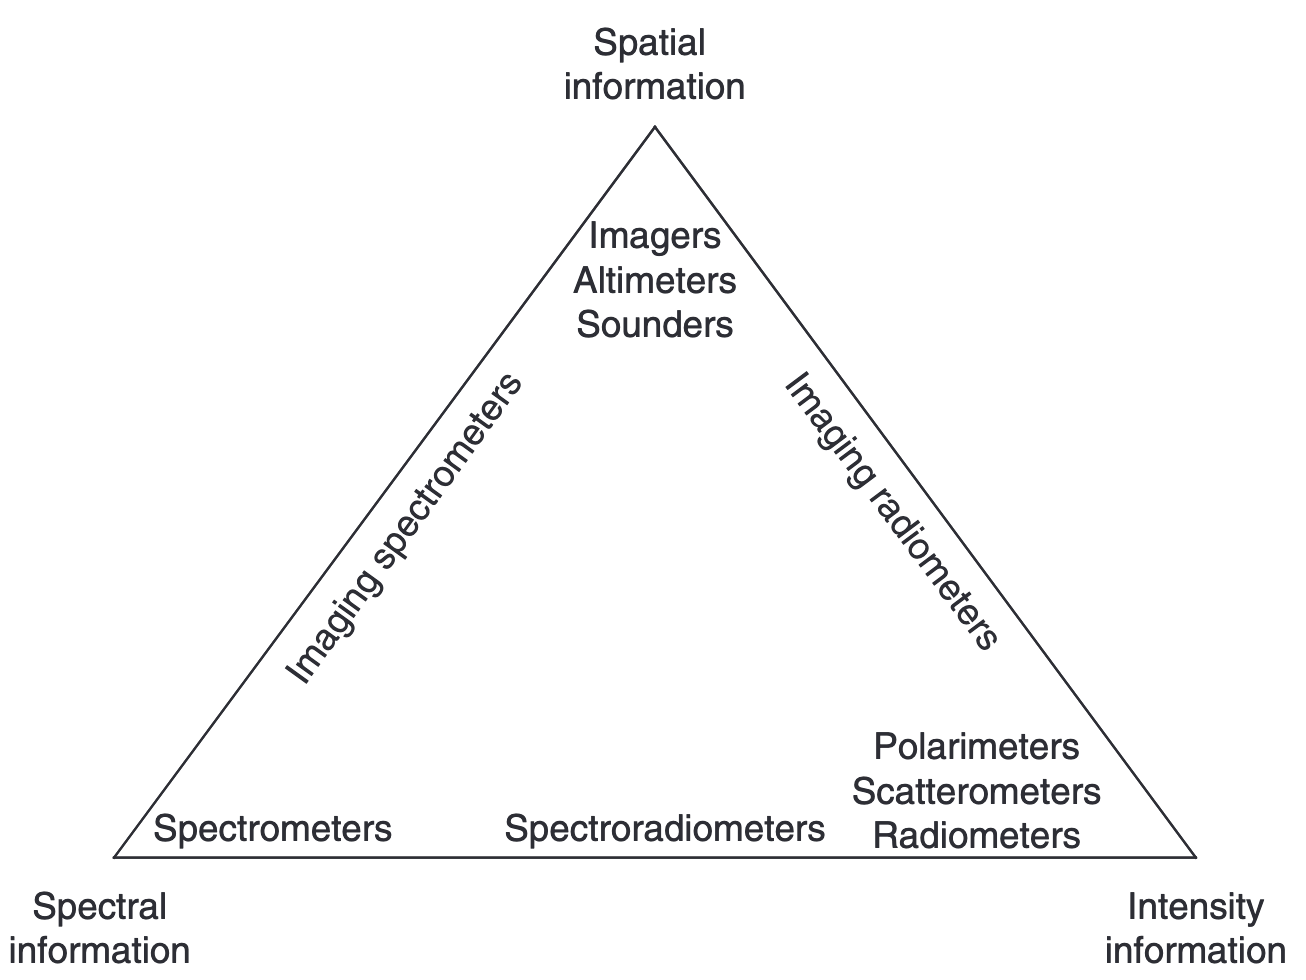
\includegraphics[width=0.6\linewidth]{images/remote-sensor-tradeoff.png}
    \caption{Placeholder for self generated version of this chart from Introduction to the Physics and Techniques of Remote Sensing.~\textsuperscript{[48]}}
    \label{figure14}
\end{figure}

% Spectrometers and radiometers

\par{Where spatial data is less of a priority, other sensors of electromagnetic radiation may be better suited to the task. Similarly to a multispectral imager, a Spectrometer divides incident electromagnetic radiation into bands, abliet much smaller ones, and discrete elements detect the intensity in each narrow band, or bin, to output a spectral plot for detailed information on spectral content.~\textsuperscript{[48]} Spectrometers are commonly used to insight into the specific chemical composition of a surface being sensed. The need for detecting chemical compositions of surfaces across a spatial extent gave rise to imaging spectrometers---an array of spectrometers.~\textsuperscript{[48]} Radiometers exist for use-cases where neither spatial nor spectral data is needed, and instead the intensity of waves across wide portions of the electromagnetic spectrum best characterizes the phenomena of interest.~\textsuperscript{[48]} Each of these sensors represents a different point on the tradeoff gradient between spectral, spatial, and intensity and information.~(\cref{figure14})~\textsuperscript{[48]}}

% Juxtaposing images of visible and infrared maps

% Thermal imaging

\par{Max Planck states in his 1914 book \textit{The Theory of Heat Radiation} that heat propagates by radiation, and moreover that heat rays are identical to light rays of the same wavelength.~\textsuperscript{[57]} It can also be said, that an object with a temperature different than absolute zero emits electromagnetic radiation.~\textsuperscript{[48]} Wein's law states that the peak wavelength of a at which an object emits the most energy is inversely proportional to that object's temperature.~\textsuperscript{[48]} Thermal imagers leverage this fact to capture an image conveying the spatial distribution of a subject's temperature to the user at a distance. Although thermal radiation occurs at wavelengths across electromagnetic spectrum, emission occurs primarily in the infrared spectrum.~\textsuperscript{[48]}~\textsuperscript{[58]} Thermal imagers (also thermal cameras / infrared cameras) purposed for remote sensing typically measure the electromagnetic radiation from the following bands---Medium Wavelength Infrared (MWIR, 3-8µm) useful for identifying high temperatures emitted by phenomena such as forrest fires or volcanic activity, and Long Wavelength Infrared (LWIR, 8-15µm) for differentiating between Earth's surface materials like soil, water, and vegetation.~\textsuperscript{[45]}~\textsuperscript{[46]}~\textsuperscript{[51]}~\textsuperscript{[52]}~\textsuperscript{[59]} From the Plank-Einstein relation it is implied that wavelength of a photon is inversely related to it's wavelength, so thermal infrared radiation is more susceptible to being attenuated by the earth's atmosphere than visible light, and is unable to penetrate cloud coverage.~\textsuperscript{[59]} On Landsat, a separate device (Thermal Infrared Scanner) is used for thermal imaging than for imaging of other parts of the electromagnetic spectrum, because the detector elements must be larger to be sensitive enough to measure the weaker signals, resulting in coarser resolution~(\cref{figure13}).~\textsuperscript{[53]}~\textsuperscript{[54]}~\textsuperscript{[59]} Thermal cameras are available at moderate cost in small footprint forms, similar to photographic cameras, and can be mounted to a large variety of platforms for remote sensing.~\textsuperscript{[54]}}

\begin{figure}
    \centering
    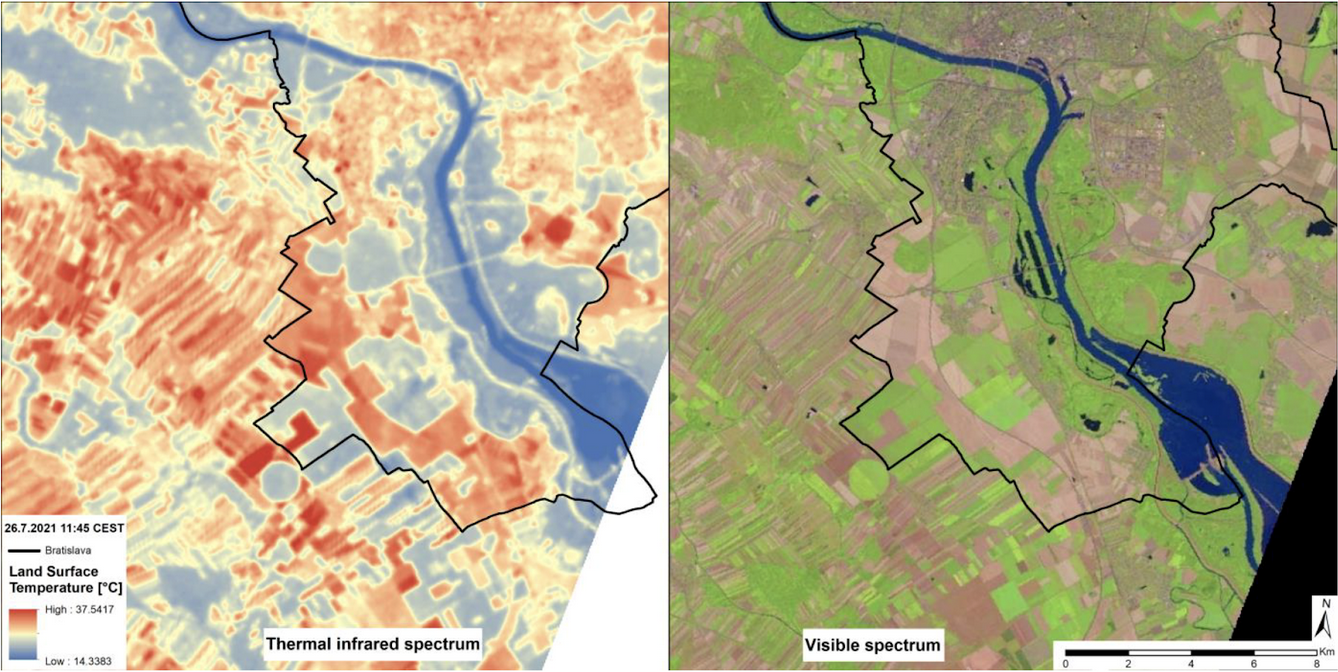
\includegraphics[width=1\linewidth]{images/thermal-vs-visible.png}
    \caption{Placeholder for self generated version of this image from An introduction to thermal infrared.~\textsuperscript{[59]}}
    \label{figure15}
\end{figure}

% Radar

\par{The first active sensor we will discuss is RADAR (Radio Detection and Ranging), a system that transmits packets in the microwave portion of the electromagnetic spectrum, receives the echo of the emitted signal off of surfaces in its surroundings, then measures the delay time to ascertain the distance of reflective surfaces from the source.~\textsuperscript{[61]}~\textsuperscript{[62]} Commonly, RADAR systems are extended to use raw sensor data in calculations that allow for the detection, location, and tracking of objects.~\textsuperscript{[48]}~\textsuperscript{[61]}~\textsuperscript{[62]} The first application of RADAR was as a aircraft detection and warning system pioneered during the Second World War, but it's role has since expanded to include a wide range of applications including, with respect to our scope---ecological, meterological, and oceanographical monitoring and survey.~\textsuperscript{[48]}~\textsuperscript{[61]}~\textsuperscript{[62]}}

% Seasat visual materials

\begin{figure}
    \centering
    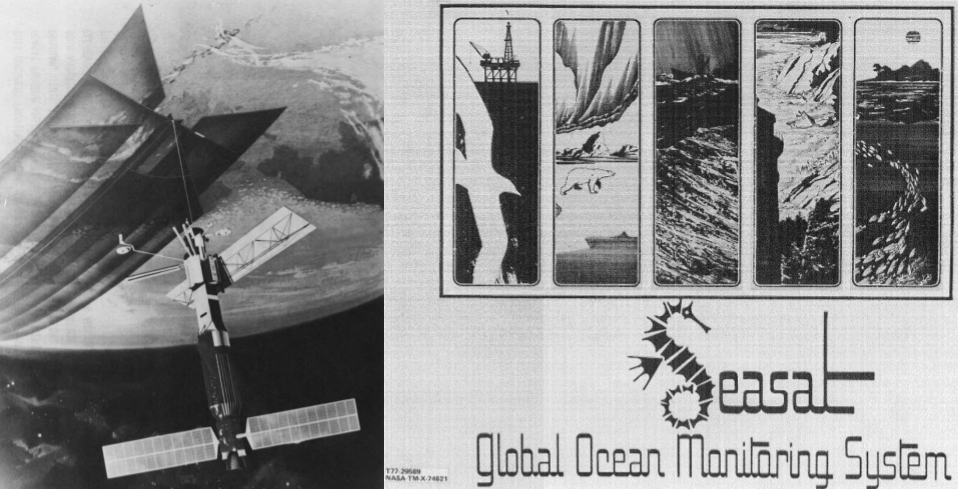
\includegraphics[width=1\linewidth]{images/seasat-material.png}
    \caption{Visual materials from documentation for the Seasat Mission.~\textsuperscript{[60]}}
    \label{figure16}
\end{figure}

% History of radar for scientific applications --- i.e. Seasat

\par{A major landmark for the implemention the RADAR for environmental remote sensing was the formation of the NASA Jet Propulsion Laberatory's Seasat program in 1973.~\textsuperscript{[48]}~\textsuperscript{[62]} Seasat is especially relevant to our scope, as the focus of the mission was to continuously gather remotely sensed data from the ocean surface for oceanographical and meterological research.~\textsuperscript{[62]} The Seasat system specifications and activities were collaboratively defined by governmental agencies, scientific bodies, and prospective users in private industry, to be able to meet use-case requirements.~\textsuperscript{[62]} Although the mission only lasted 100-days, it was able to capture more information than the past century of data gathered from ship-borne devices. For these reasons, Seasat serves as an effective basis of reference for oceanographical RADAR-based remote sensing techniques.}

% Seasat sensors

\par{Seasat contained five instruments that used RADAR in different configurations, which continue to provide a basis for modern implementations of RADAR for environmental remote sensing---a radar altimeter for geoidial altitude measurements, a microwave scatterometer to measure wind speed at the ocean's surface, a scanning multispectral microwave radiometer to measure ocean surface and ice temperatures as well as high speed winds, a visible and IR radiometer to obtain images of cloud, land, and water features, and an experimental synthetic aperture radar for surface imagery, but with the ability to function despite weather factors and sample surface spectra, especially for the mapping of ice and open water.~\textsuperscript{[62]} Unlike Landsat, Seasat did not operate in a sun synchronous orbit in order to capture diurnal variation, made possible by active RADAR sensors that emit radiation instead of capturing that of the sun reflected off of objects.~\textsuperscript{[62]} The ability for Seasat to operate day or night, in addition the large comparative swath range of it's synthetic aperture radar (1000km), allowed Seasat to achieve a 36-hour full coverage cycle, allowing better temporal resolution for characterizing ocean processes and applications with highly perishable data requirements.~\textsuperscript{[62]}}

% Seasat sensor diagrams

\begin{figure}
    \centering
    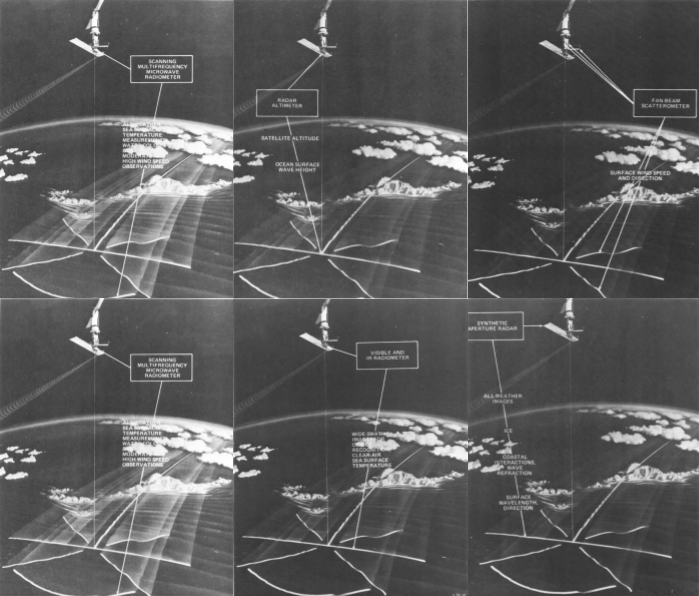
\includegraphics[width=0.8\linewidth]{images/seasat-sensors.png}
    \caption{Diagrams describing each sensor aboard Seasat.~\textsuperscript{[60]}}
    \label{figure17}
\end{figure}

% Altimeter

\par{An altimeter is used to measure the altitude of an object above a fixed level, and not all altimeters fall under the category of remote sensor.~\textsuperscript{[48]} Of interest here are RADAR altimeters, which measure the time taken for an emitted radio wave to reflect off of a surface and return.~\textsuperscript{[48]} Spaceborne altimeters are the method of choice for obtaining measurements for geodesy---the science of understanding the earth's geometric shape.~\textsuperscript{[48]}~\textsuperscript{[62]}}

% Scatterometer

\par{A RADAR scatterometer measures backscatter expressed decibels (dB), which represents the amount of a pulse that is reflected back toward the source.~\textsuperscript{[48]}  When an electromagnetic wave is incident on a surface between two materials, the radiation is scattered in different directions, some through the medium, some in all directions away from the surface, and some in the specular direction in relation to the angle of approach.~\textsuperscript{[48]} In environmental remote sensing, there are backscatter characteristics associated with certain phenomena, for example---Seasat was successful in obtaining accurate measurements of oceanic by measuring the backscatter from pulses off of capillary waves, that at certain sizes produce a high amplitude backscatter signal, as opposed to a calm ocean surface at equilibrium.~\textsuperscript{[62]}~\textsuperscript{[63]} Other radar systems }

% Visable IR / microwave radiometer
% ***** NOTE: Go into more detail about current applications *****

\par{The scanning microwave and visable / infrared radiometers aboard Seasat are similar to Landsat's Operational Land Imager device discussed earlier, insofar as they capture images of predefined bands of the electromagnetic spectrum passively.~\textsuperscript{[62]} Radiation from the microwave band (1m-1mm) of the electromagnetic spectrum can be used to derive important information about atmospheric temperature and humidity---aside from Seasat, an example of microwave radiometers being used for this purpose is Mariner 2, a NASA sponsored space probe which flew by Venus and successfully reported high surface temperatures and cool cloud coverage.~\textsuperscript{[64]} Microwave scatterometers are often deployed from the ground as well for continuous atmospheric monitoring.~\textsuperscript{[65]}~\textsuperscript{[66]} The addition of these sensors on Seasat, redundant with those on other satellites in simultaneous operation, was to provide a source of comparative data given the alternate orbit of Seasat to the other satellites that were sun sychronous.~\textsuperscript{[62]}}

% SAR example
\begin{figure}
    \centering
    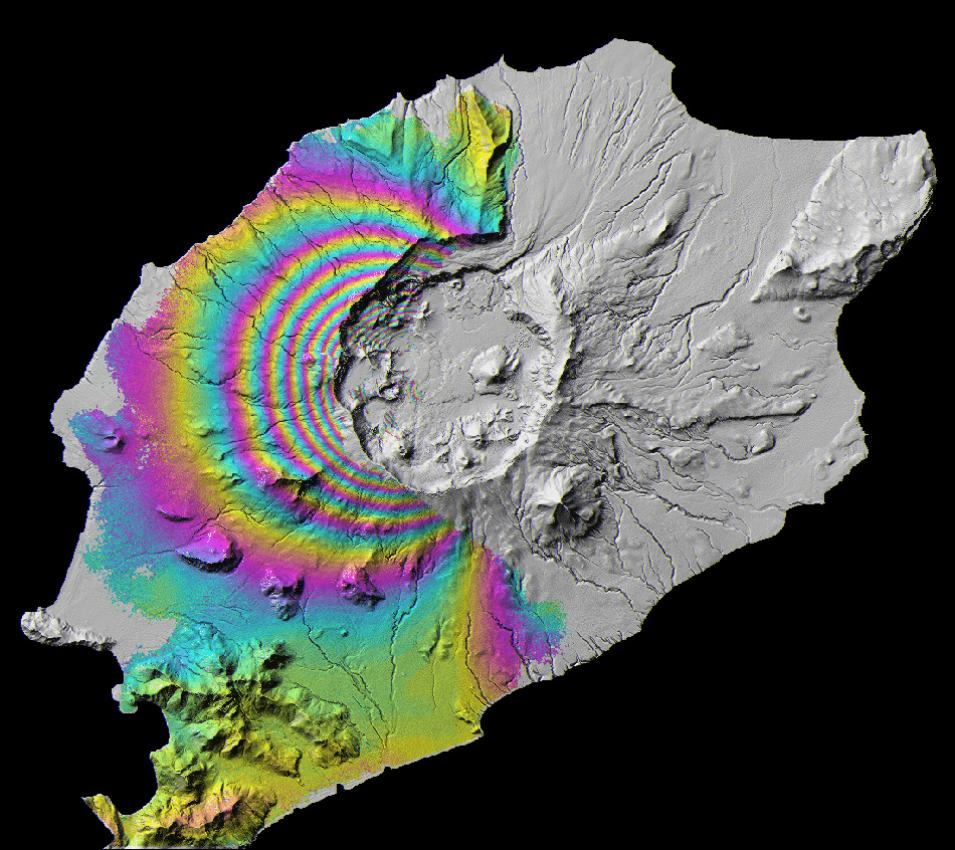
\includegraphics[width=1\linewidth]{images/sar-interferometry-okmok-volcano.jpg}
    \caption{Surface deformation on Okmok, a volcano in the Aleutian Islands, is revealed in this interferometric SAR (InSAR) ERS-2 image. Each color cycle represents 2.8 cm of ground surface movement. Credit: NASA’s Alaska Satellite Facility Distributed Active Archive Center (ASF DAAC).}
    \label{figure18}
\end{figure}

% SAR

\par{Seasat deployed the first spaceborne synthetic aperture RADAR (SAR)---but it's development and deployment on aircraft preceeds the creation of the Seasat program by a couple of decades.~\textsuperscript{[62]} SAR is a form of active radar that transmits packets and receives backscatter, measuring raw amplitude and phase data of returned radiation from a moving platform such as an aircraft of spacecraft.~\textsuperscript{[48]}~\textsuperscript{[62]}~\textsuperscript{[67]} The aperture is synthesized as the platform surveys the area of interest, each successive radar cycle contributing to the overall resolution of the image.~\textsuperscript{[48]}~\textsuperscript{[67]} This allows for a large swath range to be accomplished from the comparatively small aperature size required for deployment from an air or spacecraft.~\textsuperscript{[48]}~\textsuperscript{[67]} After calibration, each pixel in the resulting image corresponds to the backscatter coefficient of that point expressed in decibels (dB), which corresponds to the normalized reflectiveness per unit area.\textsuperscript{[69]} From the backscatter coefficient measurement, material and geometric properties can be derived for several discrete points across a targeted region.\textsuperscript{[69]} The implementation of SAR on Seasat was considered experimental, but today SAR is one of the most widely used tools in environmental remote sensing, for it's ability to obtain high resolution images from a variety of platforms, and because it is agnostic of signal attenuation caused by weather factors.~\textsuperscript{[48]}~\textsuperscript{[62]}}

% RADAR bands chart

\begin{figure}
    \centering
    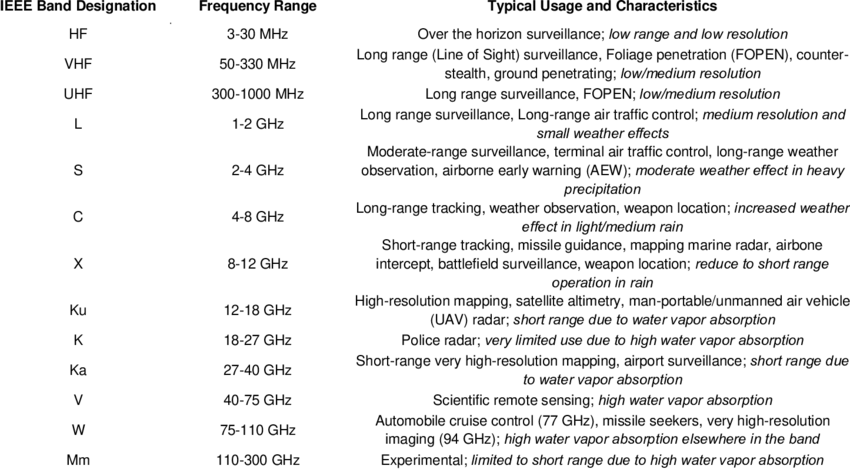
\includegraphics[width=1\linewidth]{images/radar-bands.png}
    \caption{Chart of RADAR bands and uses.~\textsuperscript{[60]}}
    \label{figure19}
\end{figure}

% RADAR Bands

\par{RADAR systems purposed for environmental remote sensing commonly use the following microwave bands for specific use-cases---the L-band (15-30cm) for biomass mapping and soil moisture measurement, S-band (8-15cm) for atmospheric percipitation measurement, C-band (4-8cm) for agricultural monitoring, wetland mapping, and detecting high frequency ocean processes, and X-band (4-2cm) for detecting medium-to-low frequency ocean processes, as well as topographical and urban mapping.~\textsuperscript{[67]} These band designators are a product of RADAR's early legacy as military technology as they were created for operational secrecy, but have since been adopted universally.~\textsuperscript{[70]} Higher frequency bands offer higher spatial resolution at the cost of higher atmospheric attenuation and less penetration.~\textsuperscript{[70]}}

% Furuno X-Band Radar at COPR

\begin{figure}
    \centering
    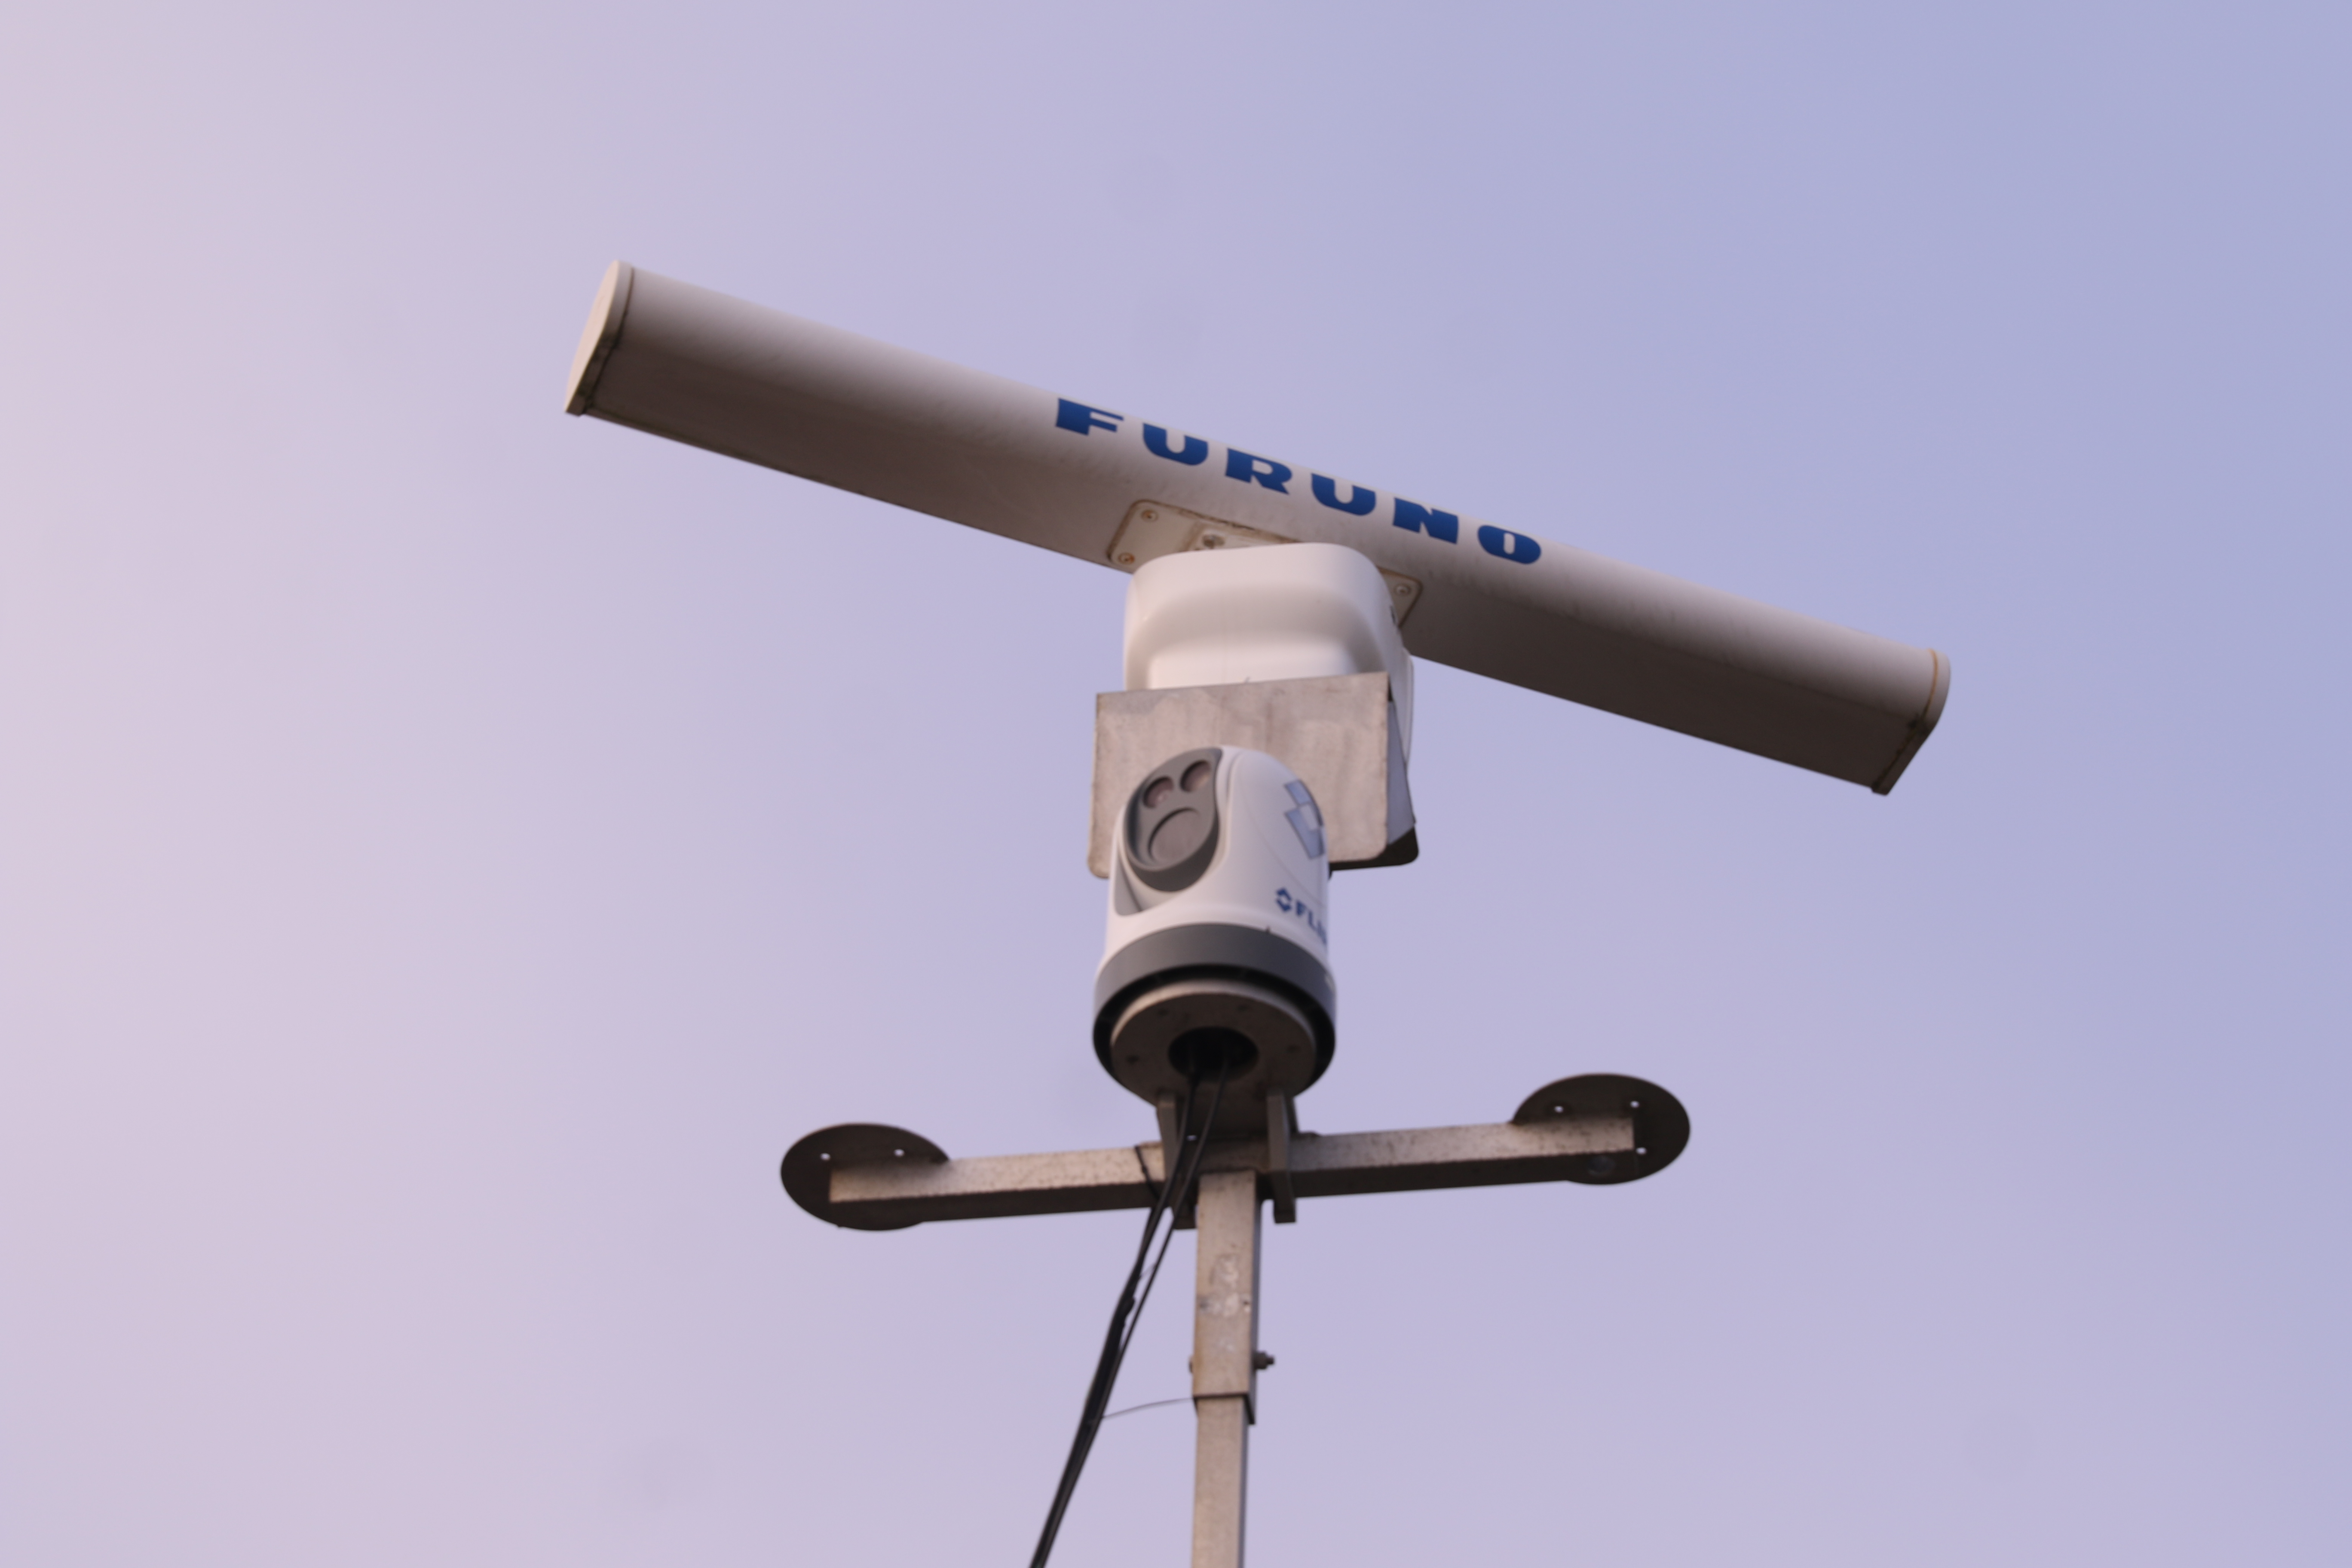
\includegraphics[width=1\linewidth]{images/furuno-x-band-radar.JPG}
    \caption{A Furuno X-Band Marine RADAR and FLIR multispectral camera system operated by NOAA at Coal Oil Point Reserve in Goleta, CA.}
    \label{figure19}
\end{figure}

% RADAR bands continued, single-band vs multiband

\par{Most RADAR systems are constrained to a single band to reduce complexity and bulk---the propagation characteristics of radiation from different bands demand different hardware specifications and signal processing algorithms. The current compliment of earth monitoring satellites deploy a variety single-band sensors---while Sentinel 1A and B deploy C-band SAR for land and ocean monitoring, ALOS 2 uses the L-band for forest and disaster monitoring.~\textsuperscript{[72]}~\textsuperscript{[73]} However, an upcoming project by NASA and the Indian Space Research Organization (ISRO) will deploy the first dual-band (L and S) SAR for unprecendentedly high-resolution (5-10m) observation of various earth processes.~\textsuperscript{[74]}

% Other platforms for RADAR
% ***** NOTE: Examples of UAVs, airborne, marine, ground *****

\par{RADAR is also deployed from a variety of airborne, shipborne, and land-based platforms. These platforms offer higher resolution and dwell, at the cost of swath range. The compactness, low-cost, and resolution of X-band RADAR makes it a popular choice for these non-spaceborne platforms.~\textsuperscript{[71]}}


% LiDAR

% Sonar --- (Single beam, multibeam, side scan, 3D)



% Ground truth comparison


% ----- 2B. TOPOGRAPHY -----
\newpage % <----- TEMPORARY
\subsection{Topography}

% Digital elevation models
% Orthographic mapping
% Dune mapping / aeolian transport
% Sentinel 1 & 2 Satellites

% ----- 2C. BATHYMETRY -----

\subsection{Bathymetry}

% Bathymetry is the missing dataset for modeling nearshore processes
% Video imagery bathymetry estimation: Stockdon and Holman 2000, Bell 1999, Aarninkhof 2003, Flampouris 2008.
% Multibeam sonar based bathymetric scanning
% Sonar Bathymetry Projects - NOAA NCEI MBES, EMODnet, IHO CSB, 
% Composite Bathymetry - GEBCO, Seabed 2023, SRTM15+
% NOAA Lidar Bathymetry

% ----- 2D. HYDROLOGY -----

\subsection{Hydrology}

% Waves from Camera: Lippmann et al 1996, Agaard and Holm 1989, Harbitz 1994, Stockdon and Holman 2000
% Wave from Radar: Izquierdo and Soares 2004
% Surface currents: Chickadel et al 2003, Puelo et al 2003, Perkovic et al 2009.
% River discharge: Passive Microwave Radiometry at Different Frequency Bands for River Discharge Retrievals
% US IOOS HF Radar
% Copernicus Marine Viewer

% ----- 2E. ECOLOGY -----

\subsection{Ecology}

% Resource investigation
% Aquatic biogeochemistry
% Biomass estimation
% Dynamic monitoring

% ----- 3. CONCLUSION -----

% ----- REFERENCE -----

\newpage
\fancyhead[C]{REFERENCE}
\fancyfoot[C]{\thepage} 
\thispagestyle{fancy}
\section{Reference}

\begin{enumerate}

    % 1
    \item {“NOAA’s National Weather Service - Glossary.” Accessed: May 01, 2025. [Online]. \href{https://forecast.weather.gov/glossary.php?word=coastal%20waters}{Available}}
    
    % 2
    \item {“Definition of the coast,” Geosciences LibreTexts. Accessed: May 01, 2025. [Online]. \href{https://geo.libretexts.org/Bookshelves/Oceanography/Coastal_Dynamics_(Bosboom_and_Stive)/01%3A_Overview/1.05%3A_Coastal_(morpho)_dynamics/1.5.01%3A_Definition_of_the_coast}{Available}}
    
    % 3
    \item {“Comparative analysis II: Land demarcation and property rights,” in ResearchGate. Accessed: May 04, 2025. [Online]. \href{https://www.researchgate.net/publication/362949604_Comparative_analysis_II_Land_demarcation_and_property_rights}{Available}}
    
    % 4
    \item {E. Hunt, M. Davidson, E. C. C. Steele, J. D. Amies, T. Scott, and P. Russell, “Shoreline modelling on timescales of days to decades,” Cambridge Prisms: Coastal Futures, vol. 1, p. e16, Jan. 2023, doi: 10.1017/cft.2023.5.}

    % 5
    \item {M. A. Davidson, K. D. Splinter, and I. L. Turner, “A simple equilibrium model for predicting shoreline change,” Coastal Engineering, vol. 73, pp. 191–202, Mar. 2013, doi: 10.1016/j.coastaleng.2012.11.002.}

    % 6
    \item {T. Garrison, Essentials of oceanography, 6th ed. Belmont, CA: Brooks/Cole, Cengage Learning, 2012.}

    % 7
    \item {R. Holman and M. C. Haller, “Remote Sensing of the Nearshore,” Annu. Rev. Mar. Sci., vol. 5, no. 1, pp. 95–113, Jan. 2013, doi: 10.1146/annurev-marine-121211-172408.}

    % 8
    \item {M. J. Kaiser and P. J. leB Williams, Eds., Marine ecology: processes, systems, and impacts, 2nd ed. Oxford; New York: Oxford University Press, 2011.}

    % 9
    \item {“Coastal Processes and Beaches | Learn Science at Scitable.” Accessed: May 05, 2025. [Online]. \href{https://www.nature.com/scitable/knowledge/library/coastal-processes-and-beaches-26276621/}{Available}}

    % 10
    \item {N. US Department of Commerce, “Marine Definitions.” Accessed: May 06, 2025. [Online]. \href{https://www.weather.gov/gum/MarineDefinitions}{Available}}

    % 11
    \item {G. Masselink, Introduction to coastal processes and geomorphology, Second edition. Oxon [England]: Routledge, 2014. doi: 10.4324/9780203785461.}

    % 12
    \item {E. B. Thornton and C. S. Kim, “Longshore current and wave height modulation at tidal frequency inside the surf zone,” Journal of Geophysical Research: Oceans, vol. 98, no. C9, pp. 16509–16519, 1993, doi: 10.1029/93JC01440.}

    % 13
    \item {T. C. Lippmann, A. H. Brookins, and E. B. Thornton, “Wave energy transformation on natural profiles,” Coastal Engineering, vol. 27, no. 1, pp. 1–20, May 1996, doi: 10.1016/0378-3839(95)00036-4.}

    % 14
    \item {B. Kinsman, Wind Waves: Their Generation and Propagation on the Ocean Surface. New York: Dover Publications, 1984.}

    % 15
    \item {W. J. Pierson Jr. and L. Moskowitz, “A proposed spectral form for fully developed wind seas based on the similarity theory of S. A. Kitaigorodskii,” Journal of Geophysical Research (1896-1977), vol. 69, no. 24, pp. 5181–5190, 1964, doi: 10.1029/JZ069i024p05181.}

    % 16
    \item {R. Davidson-Arnott, “An Introduction to Coastal Processes and Geomorphology”.}

    % 17
    \item {K. Fleming, P. Johnston, D. Zwartz, Y. Yokoyama, K. Lambeck, and J. Chappell, “Refining the eustatic sea-level curve since the Last Glacial Maximum using far- and intermediate-field sites,” Earth and Planetary Science Letters, vol. 163, no. 1, pp. 327–342, Nov. 1998, doi: 10.1016/S0012-821X(98)00198-8.}

    % 18
    \item {“Coastal prehistory in the southern Red Sea Basin, underwater archaeology, and the Farasan Islands,” ResearchGate. Accessed: May 08, 2025. [Online]. \href{https://www.researchgate.net/publication/277182725_Coastal_prehistory_in_the_southern_Red_Sea_Basin_underwater_archaeology_and_the_Farasan_Islands}{Available}}

    % 19
    \item {"N. J. Shackleton, “Oxygen isotopes, ice volume and sea level,” Quaternary Science Reviews, vol. 6, no. 3–4, pp. 183–190, Jan. 1987, doi: 10.1016/0277-3791(87)90003-5."}

    % 20
    \item {"H. Ji, S. Pan, and S. Chen, “Impact of river discharge on hydrodynamics and sedimentary processes at Yellow River Delta,” Marine Geology, vol. 425, p. 106210, Jul. 2020, doi: 10.1016/j.margeo.2020.106210."}

    % 21
    \item{"C. M. Broaddus et al., “First‐Order River Delta Morphology Is Explained by the Sediment Flux Balance From Rivers, Waves, and Tides,” Geophysical Research Letters, vol. 49, no. 22, p. e2022GL100355, Nov. 2022, doi: 10.1029/2022GL100355."}

    % 22
    \item{A. Ruiz-Reina, A. López-Ruiz, and M. Ortega-Sánchez, “River Mouth Hydrodynamics: The Role of the Outlet Geometry and Transient Tidal and River Discharge Conditions on the Jet Structure,” Journal of Geophysical Research: Oceans, vol. 130, no. 1, p. e2024JC021500, 2025, doi: 10.1029/2024JC021500.}

    % 23
    \item{K. Patsch and G. Griggs, “DEVELOPMENT OF SAND BUDGETS FOR CALIFORNIA S MAJOR LITTORAL CELLS”.}

    % 24
    \item{Littoral cells in Southern California. (Inman and Chamberlain, 1960) Accessed: May 11, 2025. [Online] \href{https://www.researchgate.net/figure/Littoral-cells-in-Southern-California-Inman-and-Chamberlain-1960-Thurman-and_fig4_240635473}{Available}}

    % 25
    \item{M. M. Alemu, “Integrated Watershed Management and Sedimentation,” Journal of Environmental Protection, vol. 7, no. 4, Art. no. 4, Mar. 2016, doi: 10.4236/jep.2016.74043.}

    % 26
    \item{A. W. Stevens et al., “Monitoring and modeling dispersal of a submerged nearshore berm at the mouth of the Columbia River, USA,” Coastal Engineering, vol. 181, p. 104285, Apr. 2023, doi: 10.1016/j.coastaleng.2023.104285.}

    % 27
    \item{W. R. Geyer, D. K. Ralston, M. C. Haller, C. Bassett, and D. Honegger, “The Structure and Dynamics of an Estuarine Tidal Intrusion Front,” Journal of Geophysical Research: Oceans, vol. 129, no. 2, p. e2023JC020371, 2024, doi: 10.1029/2023JC020371.}

    % 28
    \item{P. D. Komar, Beach processes and sedimentation. Upper Saddle River, N.J.: Prentice Hall, 1998. Accessed: May 15, 2025. [Online]. \href{http://archive.org/details/beachprocessesse0002koma}{Available}}

    % 29
    \item{T. J. O’Hare and D. A. Huntley, “Bar formation due to wave groups and associated long waves,” Marine Geology, vol. 116, no. 3–4, pp. 313–325, Feb. 1994, doi: 10.1016/0025-3227(94)90048-5.}

    % 30
    \item{C. W. T. van Bemmelen, M. A. de Schipper, J. Darnall, and S. G. J. Aarninkhof, “Beach scarp dynamics at nourished beaches,” Coastal Engineering, vol. 160, p. 103725, Sep. 2020, doi: 10.1016/j.coastaleng.2020.103725.}

    % 31
    \item{M. D. DaSilva, P. A. Hesp, D. Bruce, J. Downes, and G. M. da Silva, “Coastal transgressive dunefield evolution as a response to multi-decadal shoreline erosion,” Geomorphology, vol. 455, p. 109165, Jun. 2024, doi: 10.1016/j.geomorph.2024.109165.}

    % 32
    \item{B. Reichmüth and E. J. Anthony, “Tidal influence on the intertidal bar morphology of two contrasting macrotidal beaches,” Geomorphology, vol. 90, no. 1–2, pp. 101–114, Oct. 2007, doi: 10.1016/j.geomorph.2007.01.015.}

    % 33
    \item{Coastal Bio-Geomorphologic Zonation of Coral Reefs and Mangroves and Tide Level Control,” ResearchGate, Accessed: May 17, 2025. [Online]. \href{https://www.researchgate.net/publication/266092059_Coastal_Bio-Geomorphologic_Zonation_of_Coral_Reefs_and_Mangroves_and_Tide_Level_Control}{Available}}

    % 34
    \item{D. Morrisey, C. Beard, M. Morrison, R. Craggs, and M. Lowe, The New Zealand Mangrove: Review of the Current State of Knowledge, Auckland Regional Council, Technical Publication No. TP325, May 2007.}

    % 35
    \item{F. Ferrario, M. W. Beck, C. D. Storlazzi, F. Micheli, C. C. Shepard, and L. Airoldi, “The effectiveness of coral reefs for coastal hazard risk reduction and adaptation,” Nat Commun, vol. 5, no. 1, p. 3794, May 2014, doi: 10.1038/ncomms4794.}

    % 36
    \item{S. A. Bitterwolf, B. G. Reguero, C. D. Storlazzi, and M. W. Beck, “Shifting sands: The influence of coral reefs on shoreline erosion from short-term storm protection to long-term disequilibrium,” Nature-Based Solutions, vol. 6, p. 100174, Dec. 2024, doi: 10.1016/j.nbsj.2024.100174.}

    % 37
    \item{M. R. Gourlay, “Wave transformation on a coral reef,” Coastal Engineering, vol. 23, no. 1, pp. 17–42, May 1994, doi: 10.1016/0378-3839(94)90013-2.}

    % 38
    \item{Flood, P. (2011). Cay Formation. In: Hopley, D. (eds) Encyclopedia of Modern Coral Reefs. Encyclopedia of Earth Sciences Series. Springer, Dordrecht. https://doi.org/10.1007/978-90-481-2639-2_60}

    % 39
    \item{B. Anderson, Imagined Communities: Reflections on the Origin and Spread of Nationalism, Rev. ed. London: Verso, 1991. [Online]. \href{https://search.worldcat.org/title/880118890}{Available}}

    % 40
    \item{R. A. Schowengerdt, Remote Sensing: Models and Methods for Image Processing, 3rd ed. Amsterdam: Elsevier, 2007. [Online]. \href{https://books.google.com/books?id=KQXNaDH0X-IC&pg=PA2}{Available}}

    % 41
    \item{A. Van Dongeren, N. Plant, A. Cohen, D. Roelvink, M. C. Haller, and P. Catalán, “Beach Wizard: Nearshore bathymetry estimation through assimilation of model computations and remote observations,” Coastal Engineering, vol. 55, no. 12, pp. 1016–1027}

    % 42
    \item{“Data Assimilation.” Accessed: May 19, 2025. [Online]. \href{https://www.aoml.noaa.gov/hrd/themes/0/}{Available}}

    % 43
    \item{"P. Izquierdo and C. Guedes Soares, “Analysis of sea waves and wind from X-band radar,” Ocean Engineering, vol. 32, no. 11–12, pp. 1404–1419, Aug. 2005, doi: 10.1016/j.oceaneng.2004.11.005."}

    % 44
    \item{J. C. Nieto Borge and C. Guedes Soares, “Analysis of directional wave fields using X-band navigation radar,” Coastal Engineering, vol. 40, no. 4, pp. 375–391, Jul. 2000, doi: 10.1016/S0378-3839(00)00019-3.}

    % 45
    \item{“Landsat 8 | Landsat Science.” Accessed: May 19, 2025. [Online]. Available: https://landsat.gsfc.nasa.gov/satellites/landsat-8/}

    % 46
    \item{"M. A. Wulder et al., “Current status of Landsat program, science, and applications,” Remote Sensing of Environment, vol. 225, pp. 127–147, May 2019, doi: 10.1016/j.rse.2019.02.015."}

    % 47
    \item{"Davis, L.R., Fishburn, K.A., Lestinsky, H., Moore, L.R., and Walter, J.L., 2019, US Topo Product Standard (ver. 2.0, February 2019): U.S. Geological Survey Techniques and Methods, book 11, chap. B2, 20 p., 3 plates, scales 1:24,000, 1:25,000, and 1:20,000, https://doi.org/10.3133/tm11b2."}

    % 48
    \item{C. Elachi and J. van Zyl, “Introduction to the Physics and Techniques of Remote Sensing”.}

    % 49
    \item{S. Agrawal and G. B. Khairnar, “A COMPARATIVE ASSESSMENT OF REMOTE SENSING IMAGING TECHNIQUES: OPTICAL, SAR AND LIDAR,” Int. Arch. Photogramm. Remote Sens. Spatial Inf. Sci., vol. XLII-5/W3, pp. 1–6, Dec. 2019, doi: 10.5194/isprs-archives-XLII-5-W3-1-2019.}

    % 50
    \item{M. S. Wong, X. Zhu, S. Abbas, C. Y. T. Kwok, and M. Wang, “Optical Remote Sensing,” in Urban Informatics, W. Shi, M. F. Goodchild, M. Batty, M.-P. Kwan, and A. Zhang, Eds., Singapore: Springer, 2021, pp. 315–344. doi: 10.1007/978-981-15-8983-6_20.}

    % 51
    \item{S. N. Goward, J. G. Masek, D. L. Williams, J. R. Irons, and R. J. Thompson, “The Landsat 7 mission Terrestrial research and applications for the 21st century”.}

    % 52
    \item{“What are the band designations for the Landsat satellites? | U.S. Geological Survey.” Accessed: May 21, 2025. [Online]. \href{https://www.usgs.gov/faqs/what-are-band-designations-landsat-satellites}{Available}}

    % 53
    \item{“Landsat 8 (L8) Data Users Handbook”.}

    % 54
    \item{L. Owen, “Landsat 9 Data Users Handbook”.}

    % 55
    \item{“Taking Landsat 8 to the Beach.” Accessed: May 21, 2025. [Online] \href{https://earthobservatory.nasa.gov/images/84218/taking-landsat-8-to-the-beach}{Available}}

    % 56
    \item{“How is the Landsat 8 and Landsat 9 Coastal/Aerosol Band 1 used? | U.S. Geological Survey.” Accessed: May 21, 2025. [Online]. \href{https://www.usgs.gov/faqs/how-landsat-8-and-landsat-9-coastalaerosol-band-1-used}{Available}}

    % 57
    \item{Planck, M. The Theory of Heat Radiation. 2nd ed., translated by M. Masius, Philadelphia, PA: P. Blakiston's Son & Co., 1914.}

    % 58
    \item{J. R. Howell and R. Siegel, Thermal Radiation Heat Transfer. Volume 3: Radiation Transfer with Absorbing, Emitting, and Scattering Media, NASA Special Publication SP-164, vol. 3, Jan. 1971. [Online]. \href{https://ntrs.nasa.gov/api/citations/19710021465/downloads/19710021465.pdf}{Available}

    % 59
    \item{R. Njambi, “An introduction to thermal infrared,” UP42 Official Website. Accessed: May 24, 2025. [Online]. \href{https://up42.com/blog/introduction-to-thermal-infrared}{Available}}

    % 60
    \item{Eastwood, Eric. Radar Ornithology. London: Methuen & Co. Ltd, 1967. ISBN: 9780416442700.}

    % 61
    \item{H. Ka and M. Hasan, “STUDY ON DEVELOPMENT OF RADAR TECHNOLOGY AND IT’S FUTURE”.}

    % 62
    \item{NASA, SEASAT Global Ocean Monitoring System, NASA Technical Memorandum NASA-TM-X-74621, Jan. 1977. [Online]. \href{https://ntrs.nasa.gov/citations/19770017623}{Available}}

    % 63
    \item{W. J. Plant and W. C. Keller, "Radar returns from the sea surface—Bragg scattering and breaking waves," Journal of Physical Oceanography, vol. 18, no. 8, pp. 1065–1074, Aug. 1988. [Online]. \href{https://journals.ametsoc.org/view/journals/phoc/18/8/1520-0485_1988_018_1065_rrftss_2_0_co_2.pdf}{Available}}

    % 64
    \item{“Mariner 2 - NASA Science.” Accessed: May 30, 2025. [Online]. \href{https://science.nasa.gov/mission/mariner-2/}{Available}}

    % 65
    \item{F. T. Ulaby, R. K. Moore, and A. K. Fung, “Microwave remote sensing: Active and passive. Volume 1 - Microwave remote sensing fundamentals and radiometry.” Jan. 01, 1981. Accessed: May 30, 2025. [Online]. \href{https://ntrs.nasa.gov/citations/19820039342}{Available}}

    % 66
    \item{“Thermal Microwave Radiation - Applications for Remote Sensing,” ResearchGate. Accessed: May 30, 2025. [Online]. \href{https://www.researchgate.net/publication/234004285_Thermal_Microwave_Radiation_-_Applications_for_Remote_Sensing}{Available}}

    % 67
    \item{N. Earth Science Data Systems, “Synthetic Aperture Radar (SAR) | NASA Earthdata.” Accessed: May 26, 2025. [Online]. \href{https://www.earthdata.nasa.gov/learn/earth-observation-data-basics/sar}{Available}}

    % 68
    \item{D. Duan, Y. Wang, and Y. Zhang, “The critical role of cross-polarized backscatter in understanding L-band PolSAR data in forested and urban environments,” Remote Sensing of Environment, vol. 311, p. 114265, Sep. 2024, doi: 10.1016/j.rse.2024.114265.}

    % 69
    \item{E. Colin, “What are the physical quantities in a SAR image?,” Medium. Accessed: May 30, 2025. [Online]. \href{https://elisecolin.medium.com/what-are-the-physical-quantities-in-a-sar-image-c788a8265abd}{Available}}

    % 70
    \item{M. I. Skolnik, Introduction to radar systems, 2d ed. New York: McGraw-Hill, 1980.}

    % 71
    \item{S. Y. Matrosov, P. C. Kennedy, and R. Cifelli, “Experimentally Based Estimates of Relations between X-Band Radar Signal Attenuation Characteristics and Differential Phase in Rain,” Nov. 2014, doi: 10.1175/JTECH-D-13-00231.1.}

    % 72
    \item{“ALOS-2 / PALSAR-2.” Accessed: May 30, 2025. [Online]. \href{https://www.eorc.jaxa.jp/ALOS-2/en/about/palsar2.htm}{Available}}

    % 73
    \item{“Sentinel-1 – Documentation.” Accessed: May 30, 2025. [Online]. \href{https://documentation.dataspace.copernicus.eu/Data/SentinelMissions/Sentinel1.html}{Available}}

    % 74
    \item{“Quick Facts | Mission,” NASA-ISRO SAR Mission (NISAR). Accessed: May 30, 2025. [Online]. \href{https://nisar.jpl.nasa.gov/mission/quick-facts}{Available}}

\end{enumerate}

% ----- END -----
\end{document}